\begin{filecontents*}{simdata.dat}
t vin tp2 c1 tp3 x out
0.000 5.0000 -0.2396 9.3809 9.0016 7.8647 1.8314
0.010 5.0000 -0.2293 9.2669 8.8878 7.8313 1.7979
0.020 5.0000 -0.2190 9.1514 8.7726 7.7970 1.7635
0.030 5.0000 -0.2088 9.0347 8.6561 7.7616 1.7281
0.040 5.0000 -0.1985 8.9168 8.5385 7.7250 1.6914
0.050 5.0000 -0.1883 8.7980 8.4200 7.6867 1.6531
0.060 5.0000 -0.1781 8.6784 8.3007 7.6460 1.6125
0.070 5.0000 -0.1680 8.5580 8.1807 7.6018 1.5682
0.080 5.0000 -0.1578 8.4370 8.0601 7.5511 1.5176
0.090 5.0000 -0.1477 8.3154 7.9389 7.4891 1.4557
0.100 5.0000 -0.1376 8.1933 7.8171 7.4125 1.3794
0.110 5.0000 -0.1275 8.0707 7.6950 7.3274 1.2946
0.120 5.0000 -0.1174 7.9479 7.5725 7.2400 1.2075
0.130 5.0000 -0.1074 7.8247 7.4498 7.1516 1.1195
0.140 5.0000 -0.0974 7.7013 7.3268 7.0625 1.0307
0.150 5.0000 -0.0874 7.5778 7.2037 6.9723 0.9408
0.160 5.0000 -0.0774 7.4541 7.0805 6.8803 0.8493
0.170 5.0000 -0.0675 7.3303 6.9572 6.7847 0.7541
0.180 5.0000 -0.0575 7.2063 6.8337 6.6814 0.6514
0.190 5.0000 -0.0476 7.0823 6.7102 6.5694 0.5400
0.200 5.0000 -0.0377 6.9583 6.5866 6.4546 0.4259
0.210 5.0000 -0.0279 6.8342 6.4631 6.3396 0.3116
0.220 5.0000 -0.0180 6.7102 6.3396 6.2246 0.1973
0.230 5.0000 -0.0082 6.5862 6.2162 6.1097 0.0831
0.240 5.0000 0.0016 6.4623 6.0929 5.9948 -0.0309
0.250 5.0000 0.0114 6.3385 5.9697 5.8801 -0.1449
0.260 5.0000 0.0212 6.2148 5.8466 5.7655 -0.2586
0.270 5.0000 0.0309 6.0911 5.7237 5.6510 -0.3722
0.280 5.0000 0.0406 5.9676 5.6009 5.5367 -0.4856
0.290 5.0000 0.0503 5.8443 5.4782 5.4229 -0.5984
0.300 5.0000 0.0600 5.7211 5.3558 5.3124 -0.7079
0.310 5.0000 0.0697 5.5981 5.2336 5.2109 -0.8084
0.320 5.0000 0.0793 5.4753 5.1117 5.1168 -0.9016
0.330 5.0000 0.0889 5.3527 4.9901 5.0262 -0.9913
0.340 5.0000 0.0985 5.2303 4.8687 4.9373 -1.0792
0.350 5.0000 0.1081 5.1081 4.7475 4.8496 -1.1660
0.360 5.0000 0.1177 4.9861 4.6266 4.7627 -1.2519
0.370 5.0000 0.1272 4.8643 4.5059 4.6766 -1.3369
0.380 5.0000 0.1367 4.7427 4.3855 4.5928 -1.4196
0.390 5.0000 0.1462 4.6214 4.2654 4.5169 -1.4946
0.400 5.0000 0.1557 4.5003 4.1458 4.4549 -1.5557
0.410 5.0000 0.1652 4.3796 4.0266 4.4043 -1.6055
0.420 5.0000 0.1746 4.2591 3.9078 4.3602 -1.6489
0.430 5.0000 0.1840 4.1389 3.7894 4.3197 -1.6887
0.440 5.0000 0.1934 4.0189 3.6713 4.2814 -1.7264
0.450 5.0000 0.2028 3.8992 3.5536 4.2446 -1.7625
0.460 5.0000 0.2121 3.7797 3.4362 4.2089 -1.7976
0.470 5.0000 0.2215 3.6605 3.3193 4.1740 -1.8318
0.480 5.0000 0.2308 3.5416 3.2029 4.1398 -1.8654
0.490 5.0000 0.2401 3.4229 3.0868 4.1061 -1.8984
0.500 -5.0000 0.2396 3.4320 3.0961 4.1087 -1.8955
0.510 -5.0000 0.2293 3.5683 3.2300 4.1477 -1.8568
0.520 -5.0000 0.2190 3.7041 3.3638 4.1872 -1.8176
0.530 -5.0000 0.2088 3.8394 3.4972 4.2274 -1.7777
0.540 -5.0000 0.1985 3.9741 3.6302 4.2686 -1.7368
0.550 -5.0000 0.1883 4.1084 3.7629 4.3113 -1.6944
0.560 -5.0000 0.1781 4.2422 3.8952 4.3564 -1.6496
0.570 -5.0000 0.1680 4.3755 4.0271 4.4056 -1.6007
0.580 -5.0000 0.1578 4.5082 4.1587 4.4629 -1.5439
0.590 -5.0000 0.1477 4.6406 4.2899 4.5346 -1.4728
0.600 -5.0000 0.1376 4.7724 4.4208 4.6212 -1.3869
0.610 -5.0000 0.1275 4.9038 4.5513 4.7135 -1.2955
0.620 -5.0000 0.1174 5.0346 4.6813 4.8067 -1.2030
0.630 -5.0000 0.1074 5.1649 4.8107 4.9003 -1.1102
0.640 -5.0000 0.0974 5.2946 4.9397 4.9943 -1.0169
0.650 -5.0000 0.0874 5.4237 5.0681 5.0894 -0.9226
0.660 -5.0000 0.0774 5.5524 5.1959 5.1871 -0.8256
0.670 -5.0000 0.0675 5.6804 5.3233 5.2911 -0.7225
0.680 -5.0000 0.0575 5.8080 5.4502 5.4044 -0.6100
0.690 -5.0000 0.0476 5.9349 5.5766 5.5216 -0.4937
0.700 -5.0000 0.0377 6.0613 5.7024 5.6387 -0.3775
0.710 -5.0000 0.0279 6.1871 5.8275 5.7553 -0.2617
0.720 -5.0000 0.0180 6.3123 5.9521 5.8713 -0.1465
0.730 -5.0000 0.0082 6.4368 6.0760 5.9867 -0.0319
0.740 -5.0000 -0.0016 6.5608 6.1994 6.1015 0.0821
0.750 -5.0000 -0.0114 6.6840 6.3220 6.2158 0.1956
0.760 -5.0000 -0.0212 6.8066 6.4441 6.3294 0.3084
0.770 -5.0000 -0.0309 6.9286 6.5654 6.4424 0.4206
0.780 -5.0000 -0.0406 7.0499 6.6861 6.5545 0.5320
0.790 -5.0000 -0.0503 7.1704 6.8060 6.6639 0.6406
0.800 -5.0000 -0.0600 7.2902 6.9252 6.7650 0.7411
0.810 -5.0000 -0.0697 7.4093 7.0436 6.8578 0.8332
0.820 -5.0000 -0.0793 7.5276 7.1612 6.9461 0.9209
0.830 -5.0000 -0.0889 7.6450 7.2780 7.0319 1.0062
0.840 -5.0000 -0.0985 7.7617 7.3940 7.1162 1.0898
0.850 -5.0000 -0.1081 7.8776 7.5092 7.1992 1.1723
0.860 -5.0000 -0.1177 7.9926 7.6235 7.2811 1.2535
0.870 -5.0000 -0.1272 8.1067 7.7369 7.3614 1.3332
0.880 -5.0000 -0.1367 8.2199 7.8494 7.4377 1.4089
0.890 -5.0000 -0.1462 8.3321 7.9609 7.5040 1.4748
0.900 -5.0000 -0.1557 8.4433 8.0713 7.5578 1.5281
0.910 -5.0000 -0.1651 8.5533 8.1806 7.6027 1.5726
0.920 -5.0000 -0.1746 8.6623 8.2887 7.6424 1.6119
0.930 -5.0000 -0.1840 8.7701 8.3957 7.6790 1.6481
0.940 -5.0000 -0.1934 8.8766 8.5015 7.7134 1.6821
0.950 -5.0000 -0.2028 8.9819 8.6060 7.7463 1.7146
0.960 -5.0000 -0.2121 9.0858 8.7091 7.7779 1.7458
0.970 -5.0000 -0.2215 9.1883 8.8108 7.8085 1.7760
0.980 -5.0000 -0.2308 9.2892 8.9109 7.8381 1.8054
0.990 -5.0000 -0.2401 9.3884 9.0093 7.8670 1.8338
1.000 5.0000 -0.2396 9.3809 9.0016 7.8647 1.8314
1.010 5.0000 -0.2293 9.2669 8.8878 7.8313 1.7979
1.020 5.0000 -0.2190 9.1514 8.7726 7.7970 1.7635
1.030 5.0000 -0.2088 9.0347 8.6561 7.7616 1.7281
1.040 5.0000 -0.1985 8.9168 8.5385 7.7250 1.6914
1.050 5.0000 -0.1883 8.7980 8.4200 7.6867 1.6531
1.060 5.0000 -0.1781 8.6784 8.3007 7.6460 1.6125
1.070 5.0000 -0.1680 8.5580 8.1807 7.6018 1.5682
1.080 5.0000 -0.1578 8.4370 8.0601 7.5511 1.5176
1.090 5.0000 -0.1477 8.3154 7.9389 7.4891 1.4557
1.100 5.0000 -0.1376 8.1933 7.8171 7.4125 1.3794
1.110 5.0000 -0.1275 8.0707 7.6950 7.3274 1.2946
1.120 5.0000 -0.1174 7.9478 7.5725 7.2400 1.2075
1.130 5.0000 -0.1074 7.8247 7.4498 7.1516 1.1195
1.140 5.0000 -0.0974 7.7013 7.3268 7.0625 1.0307
1.150 5.0000 -0.0874 7.5778 7.2037 6.9723 0.9408
1.160 5.0000 -0.0774 7.4541 7.0805 6.8803 0.8493
1.170 5.0000 -0.0675 7.3303 6.9572 6.7847 0.7541
1.180 5.0000 -0.0575 7.2063 6.8337 6.6814 0.6514
1.190 5.0000 -0.0476 7.0823 6.7102 6.5694 0.5400
1.200 5.0000 -0.0377 6.9583 6.5866 6.4546 0.4259
1.210 5.0000 -0.0279 6.8342 6.4631 6.3396 0.3116
1.220 5.0000 -0.0180 6.7102 6.3396 6.2246 0.1973
1.230 5.0000 -0.0082 6.5862 6.2162 6.1097 0.0831
1.240 5.0000 0.0016 6.4623 6.0929 5.9948 -0.0309
1.250 5.0000 0.0114 6.3385 5.9697 5.8801 -0.1449
1.260 5.0000 0.0212 6.2148 5.8466 5.7655 -0.2586
1.270 5.0000 0.0309 6.0911 5.7237 5.6510 -0.3722
1.280 5.0000 0.0406 5.9676 5.6009 5.5367 -0.4856
1.290 5.0000 0.0503 5.8443 5.4782 5.4229 -0.5984
1.300 5.0000 0.0600 5.7211 5.3558 5.3124 -0.7079
1.310 5.0000 0.0697 5.5981 5.2336 5.2109 -0.8084
1.320 5.0000 0.0793 5.4753 5.1117 5.1168 -0.9016
1.330 5.0000 0.0889 5.3527 4.9901 5.0262 -0.9913
1.340 5.0000 0.0985 5.2303 4.8687 4.9373 -1.0792
1.350 5.0000 0.1081 5.1081 4.7475 4.8496 -1.1660
1.360 5.0000 0.1177 4.9861 4.6266 4.7627 -1.2519
1.370 5.0000 0.1272 4.8643 4.5059 4.6766 -1.3369
1.380 5.0000 0.1367 4.7427 4.3855 4.5928 -1.4196
1.390 5.0000 0.1462 4.6213 4.2654 4.5169 -1.4946
1.400 5.0000 0.1557 4.5003 4.1458 4.4549 -1.5557
1.410 5.0000 0.1652 4.3796 4.0266 4.4043 -1.6055
1.420 5.0000 0.1746 4.2591 3.9078 4.3602 -1.6489
1.430 5.0000 0.1840 4.1389 3.7894 4.3197 -1.6887
1.440 5.0000 0.1934 4.0189 3.6713 4.2814 -1.7264
1.450 5.0000 0.2028 3.8992 3.5536 4.2446 -1.7625
1.460 5.0000 0.2121 3.7797 3.4363 4.2089 -1.7976
1.470 5.0000 0.2215 3.6605 3.3193 4.1740 -1.8318
1.480 5.0000 0.2308 3.5416 3.2029 4.1398 -1.8654
1.490 5.0000 0.2401 3.4229 3.0868 4.1061 -1.8984
1.500 -5.0000 0.2396 3.4320 3.0961 4.1087 -1.8955
1.510 -5.0000 0.2293 3.5683 3.2301 4.1477 -1.8568
1.520 -5.0000 0.2190 3.7041 3.3638 4.1872 -1.8176
1.530 -5.0000 0.2088 3.8394 3.4972 4.2274 -1.7777
1.540 -5.0000 0.1985 3.9741 3.6302 4.2686 -1.7368
1.550 -5.0000 0.1883 4.1084 3.7629 4.3113 -1.6944
1.560 -5.0000 0.1781 4.2422 3.8952 4.3564 -1.6496
1.570 -5.0000 0.1680 4.3755 4.0271 4.4056 -1.6007
1.580 -5.0000 0.1578 4.5082 4.1587 4.4629 -1.5439
1.590 -5.0000 0.1477 4.6406 4.2899 4.5346 -1.4728
1.600 -5.0000 0.1376 4.7724 4.4209 4.6212 -1.3869
1.610 -5.0000 0.1275 4.9038 4.5513 4.7135 -1.2955
1.620 -5.0000 0.1174 5.0346 4.6813 4.8067 -1.2030
1.630 -5.0000 0.1074 5.1649 4.8107 4.9003 -1.1102
1.640 -5.0000 0.0974 5.2946 4.9397 4.9943 -1.0169
1.650 -5.0000 0.0874 5.4237 5.0681 5.0894 -0.9226
1.660 -5.0000 0.0774 5.5524 5.1960 5.1871 -0.8256
1.670 -5.0000 0.0675 5.6804 5.3233 5.2911 -0.7225
1.680 -5.0000 0.0575 5.8080 5.4502 5.4044 -0.6100
1.690 -5.0000 0.0476 5.9349 5.5766 5.5216 -0.4937
1.700 -5.0000 0.0377 6.0613 5.7024 5.6387 -0.3775
1.710 -5.0000 0.0279 6.1871 5.8275 5.7553 -0.2617
1.720 -5.0000 0.0180 6.3123 5.9521 5.8713 -0.1465
1.730 -5.0000 0.0082 6.4368 6.0761 5.9867 -0.0319
1.740 -5.0000 -0.0016 6.5607 6.1994 6.1015 0.0821
1.750 -5.0000 -0.0114 6.6840 6.3220 6.2158 0.1956
1.760 -5.0000 -0.0212 6.8066 6.4441 6.3294 0.3084
1.770 -5.0000 -0.0309 6.9286 6.5654 6.4424 0.4206
1.780 -5.0000 -0.0406 7.0499 6.6861 6.5545 0.5320
1.790 -5.0000 -0.0503 7.1704 6.8060 6.6639 0.6406
1.800 -5.0000 -0.0600 7.2902 6.9252 6.7650 0.7411
1.810 -5.0000 -0.0697 7.4093 7.0436 6.8578 0.8332
1.820 -5.0000 -0.0793 7.5276 7.1612 6.9461 0.9209
1.830 -5.0000 -0.0889 7.6450 7.2780 7.0319 1.0062
1.840 -5.0000 -0.0985 7.7617 7.3940 7.1162 1.0898
1.850 -5.0000 -0.1081 7.8776 7.5092 7.1992 1.1723
1.860 -5.0000 -0.1177 7.9926 7.6235 7.2811 1.2535
1.870 -5.0000 -0.1272 8.1067 7.7369 7.3614 1.3332
1.880 -5.0000 -0.1367 8.2199 7.8494 7.4377 1.4089
1.890 -5.0000 -0.1462 8.3321 7.9609 7.5040 1.4748
1.900 -5.0000 -0.1557 8.4433 8.0713 7.5578 1.5281
1.910 -5.0000 -0.1651 8.5533 8.1806 7.6027 1.5726
1.920 -5.0000 -0.1746 8.6623 8.2887 7.6424 1.6119
1.930 -5.0000 -0.1840 8.7701 8.3957 7.6790 1.6481
1.940 -5.0000 -0.1934 8.8766 8.5015 7.7134 1.6821
1.950 -5.0000 -0.2028 8.9819 8.6060 7.7463 1.7146
1.960 -5.0000 -0.2121 9.0858 8.7091 7.7779 1.7458
1.970 -5.0000 -0.2215 9.1883 8.8108 7.8085 1.7761
1.980 -5.0000 -0.2308 9.2892 8.9109 7.8381 1.8054
1.990 -5.0000 -0.2401 9.3884 9.0093 7.8670 1.8338
2.000 5.0000 -0.2396 9.3809 9.0016 7.8647 1.8314
2.010 5.0000 -0.2293 9.2669 8.8878 7.8313 1.7979
2.020 5.0000 -0.2190 9.1514 8.7726 7.7970 1.7635
2.030 5.0000 -0.2088 9.0347 8.6561 7.7616 1.7281
2.040 5.0000 -0.1985 8.9168 8.5385 7.7250 1.6914
2.050 5.0000 -0.1883 8.7980 8.4200 7.6867 1.6531
2.060 5.0000 -0.1781 8.6783 8.3007 7.6460 1.6125
2.070 5.0000 -0.1680 8.5580 8.1807 7.6018 1.5682
2.080 5.0000 -0.1578 8.4370 8.0601 7.5511 1.5176
2.090 5.0000 -0.1477 8.3154 7.9389 7.4891 1.4557
2.100 5.0000 -0.1376 8.1933 7.8171 7.4125 1.3794
2.110 5.0000 -0.1275 8.0707 7.6950 7.3274 1.2946
2.120 5.0000 -0.1174 7.9478 7.5725 7.2400 1.2075
2.130 5.0000 -0.1074 7.8247 7.4498 7.1516 1.1195
2.140 5.0000 -0.0974 7.7013 7.3268 7.0625 1.0307
2.150 5.0000 -0.0874 7.5778 7.2037 6.9723 0.9408
2.160 5.0000 -0.0774 7.4541 7.0805 6.8803 0.8493
2.170 5.0000 -0.0675 7.3303 6.9572 6.7847 0.7541
2.180 5.0000 -0.0575 7.2063 6.8337 6.6814 0.6514
2.190 5.0000 -0.0476 7.0823 6.7102 6.5694 0.5400
2.200 5.0000 -0.0377 6.9583 6.5866 6.4546 0.4259
2.210 5.0000 -0.0279 6.8342 6.4631 6.3396 0.3116
2.220 5.0000 -0.0180 6.7102 6.3396 6.2246 0.1973
2.230 5.0000 -0.0082 6.5862 6.2162 6.1097 0.0831
2.240 5.0000 0.0016 6.4623 6.0929 5.9948 -0.0309
2.250 5.0000 0.0114 6.3385 5.9697 5.8801 -0.1449
2.260 5.0000 0.0212 6.2148 5.8466 5.7655 -0.2586
2.270 5.0000 0.0309 6.0911 5.7237 5.6510 -0.3722
2.280 5.0000 0.0406 5.9676 5.6009 5.5367 -0.4856
2.290 5.0000 0.0503 5.8443 5.4782 5.4229 -0.5984
2.300 5.0000 0.0600 5.7211 5.3558 5.3124 -0.7079
2.310 5.0000 0.0697 5.5981 5.2336 5.2110 -0.8084
2.320 5.0000 0.0793 5.4753 5.1117 5.1168 -0.9016
2.330 5.0000 0.0889 5.3527 4.9901 5.0262 -0.9913
2.340 5.0000 0.0985 5.2303 4.8687 4.9373 -1.0792
2.350 5.0000 0.1081 5.1081 4.7475 4.8496 -1.1660
2.360 5.0000 0.1177 4.9861 4.6266 4.7627 -1.2519
2.370 5.0000 0.1272 4.8642 4.5059 4.6766 -1.3369
2.380 5.0000 0.1367 4.7427 4.3855 4.5928 -1.4196
2.390 5.0000 0.1462 4.6213 4.2654 4.5169 -1.4946
2.400 5.0000 0.1557 4.5003 4.1458 4.4549 -1.5557
2.410 5.0000 0.1652 4.3796 4.0266 4.4043 -1.6055
2.420 5.0000 0.1746 4.2591 3.9078 4.3602 -1.6489
2.430 5.0000 0.1840 4.1389 3.7894 4.3197 -1.6887
2.440 5.0000 0.1934 4.0189 3.6713 4.2814 -1.7264
2.450 5.0000 0.2028 3.8992 3.5536 4.2446 -1.7625
2.460 5.0000 0.2121 3.7797 3.4363 4.2089 -1.7975
2.470 5.0000 0.2215 3.6605 3.3193 4.1740 -1.8318
2.480 5.0000 0.2308 3.5416 3.2029 4.1398 -1.8654
2.490 5.0000 0.2401 3.4229 3.0868 4.1061 -1.8984
2.500 -5.0000 0.2396 3.4320 3.0961 4.1087 -1.8955
2.510 -5.0000 0.2293 3.5683 3.2301 4.1477 -1.8568
2.520 -5.0000 0.2190 3.7041 3.3638 4.1872 -1.8176
2.530 -5.0000 0.2088 3.8394 3.4972 4.2274 -1.7777
2.540 -5.0000 0.1985 3.9741 3.6302 4.2686 -1.7368
2.550 -5.0000 0.1883 4.1084 3.7629 4.3113 -1.6944
2.560 -5.0000 0.1781 4.2422 3.8952 4.3564 -1.6496
2.570 -5.0000 0.1680 4.3755 4.0271 4.4056 -1.6007
2.580 -5.0000 0.1578 4.5082 4.1587 4.4629 -1.5439
2.590 -5.0000 0.1477 4.6406 4.2899 4.5346 -1.4728
2.600 -5.0000 0.1376 4.7724 4.4209 4.6212 -1.3869
2.610 -5.0000 0.1275 4.9038 4.5513 4.7135 -1.2955
2.620 -5.0000 0.1174 5.0346 4.6813 4.8067 -1.2030
2.630 -5.0000 0.1074 5.1649 4.8108 4.9003 -1.1102
2.640 -5.0000 0.0974 5.2946 4.9397 4.9943 -1.0169
2.650 -5.0000 0.0874 5.4237 5.0681 5.0894 -0.9226
2.660 -5.0000 0.0774 5.5524 5.1960 5.1871 -0.8256
2.670 -5.0000 0.0675 5.6804 5.3233 5.2911 -0.7225
2.680 -5.0000 0.0575 5.8080 5.4502 5.4044 -0.6100
2.690 -5.0000 0.0476 5.9349 5.5766 5.5216 -0.4937
2.700 -5.0000 0.0377 6.0613 5.7024 5.6387 -0.3775
2.710 -5.0000 0.0279 6.1871 5.8275 5.7553 -0.2617
2.720 -5.0000 0.0180 6.3123 5.9521 5.8713 -0.1465
2.730 -5.0000 0.0082 6.4368 6.0761 5.9867 -0.0319
2.740 -5.0000 -0.0016 6.5607 6.1994 6.1015 0.0821
2.750 -5.0000 -0.0114 6.6840 6.3220 6.2158 0.1956
2.760 -5.0000 -0.0212 6.8066 6.4441 6.3294 0.3084
2.770 -5.0000 -0.0309 6.9286 6.5654 6.4424 0.4206
2.780 -5.0000 -0.0406 7.0499 6.6861 6.5545 0.5320
2.790 -5.0000 -0.0503 7.1704 6.8060 6.6639 0.6406
2.800 -5.0000 -0.0600 7.2902 6.9252 6.7650 0.7411
2.810 -5.0000 -0.0697 7.4093 7.0436 6.8578 0.8332
2.820 -5.0000 -0.0793 7.5275 7.1612 6.9461 0.9209
2.830 -5.0000 -0.0889 7.6450 7.2780 7.0319 1.0062
2.840 -5.0000 -0.0985 7.7617 7.3940 7.1162 1.0898
2.850 -5.0000 -0.1081 7.8776 7.5092 7.1992 1.1723
2.860 -5.0000 -0.1177 7.9926 7.6235 7.2811 1.2535
2.870 -5.0000 -0.1272 8.1067 7.7369 7.3614 1.3332
2.880 -5.0000 -0.1367 8.2199 7.8494 7.4377 1.4089
2.890 -5.0000 -0.1462 8.3321 7.9609 7.5040 1.4748
2.900 -5.0000 -0.1557 8.4433 8.0713 7.5578 1.5281
2.910 -5.0000 -0.1651 8.5533 8.1806 7.6027 1.5726
2.920 -5.0000 -0.1746 8.6623 8.2887 7.6424 1.6119
2.930 -5.0000 -0.1840 8.7701 8.3957 7.6790 1.6481
2.940 -5.0000 -0.1934 8.8766 8.5015 7.7134 1.6821
2.950 -5.0000 -0.2028 8.9819 8.6060 7.7463 1.7146
2.960 -5.0000 -0.2121 9.0858 8.7091 7.7779 1.7458
2.970 -5.0000 -0.2215 9.1883 8.8108 7.8085 1.7761
2.980 -5.0000 -0.2308 9.2892 8.9109 7.8381 1.8054
2.990 -5.0000 -0.2401 9.3884 9.0093 7.8670 1.8338
\end{filecontents*}
\begin{filecontents*}{psudata.dat}
t dc vcc
0.000 16.0913 12.0130
0.040 16.0884 12.0122
0.080 16.0855 12.0116
0.120 16.0826 12.0111
0.160 16.0797 12.0107
0.200 16.0768 12.0105
0.240 16.0740 12.0104
0.280 16.0711 12.0104
0.320 16.0682 12.0105
0.360 16.0653 12.0108
0.400 16.0625 12.0112
0.440 16.0596 12.0116
0.480 16.0567 12.0121
0.520 16.0538 12.0126
0.560 16.0510 12.0130
0.600 16.0481 12.0132
0.640 16.0453 12.0133
0.680 16.0424 12.0132
0.720 16.0395 12.0130
0.760 16.0367 12.0126
0.800 16.0338 12.0122
0.840 16.0310 12.0116
0.880 16.0281 12.0109
0.920 16.0253 12.0102
0.960 16.0224 12.0093
1.000 16.0196 12.0085
1.040 16.0168 12.0077
1.080 16.0139 12.0070
1.120 16.0111 12.0065
1.160 16.0082 12.0061
1.200 16.0054 12.0059
1.240 16.0026 12.0058
1.280 15.9997 12.0058
1.320 15.9969 12.0060
1.360 15.9941 12.0062
1.400 15.9912 12.0066
1.440 15.9884 12.0070
1.480 15.9856 12.0075
1.520 15.9828 12.0080
1.560 15.9799 12.0084
1.600 15.9771 12.0086
1.640 15.9743 12.0087
1.680 15.9715 12.0086
1.720 15.9687 12.0084
1.760 15.9659 12.0081
1.800 15.9631 12.0076
1.840 15.9603 12.0070
1.880 15.9575 12.0063
1.920 15.9547 12.0056
1.960 15.9519 12.0048
2.000 15.9491 12.0039
2.040 15.9463 12.0031
2.080 15.9435 12.0024
2.120 15.9407 12.0019
2.160 15.9379 12.0015
2.200 15.9351 12.0013
2.240 15.9323 12.0012
2.280 15.9295 12.0012
2.320 15.9267 12.0014
2.360 15.9240 12.0016
2.400 15.9212 12.0020
2.440 15.9184 12.0024
2.480 15.9156 12.0029
2.520 15.9129 12.0034
2.560 15.9101 12.0038
2.600 15.9073 12.0040
2.640 15.9045 12.0041
2.680 15.9018 12.0040
2.720 15.8990 12.0038
2.760 15.8963 12.0034
2.800 15.8935 12.0030
2.840 15.8907 12.0024
2.880 15.8880 12.0017
2.920 15.8852 12.0010
2.960 15.8825 12.0001
3.000 15.8797 11.9993
3.040 15.8770 11.9985
3.080 15.8742 11.9978
3.120 15.8715 11.9973
3.160 15.8687 11.9969
3.200 15.8660 11.9967
3.240 15.8632 11.9965
3.280 15.8605 11.9966
3.320 15.8578 11.9967
3.360 15.8550 11.9970
3.400 15.8523 11.9973
3.440 15.8495 11.9977
3.480 15.8468 11.9982
3.520 15.8441 11.9988
3.560 15.8414 11.9991
3.600 15.8386 11.9993
3.640 15.8359 11.9994
3.680 15.8332 11.9993
3.720 15.8305 11.9991
3.760 15.8278 11.9988
3.800 15.8251 11.9983
3.840 15.8223 11.9978
3.880 15.8196 11.9971
3.920 15.8169 11.9963
3.960 15.8142 11.9955
4.000 15.8115 11.9946
4.040 15.8090 11.9938
4.080 15.8071 11.9931
4.120 15.8084 11.9926
4.160 15.8196 11.9923
4.200 15.8463 11.9921
4.240 15.8854 11.9923
4.280 15.9303 11.9926
4.320 15.9764 11.9933
4.360 16.0217 11.9942
4.400 16.0652 11.9953
4.440 16.1065 11.9966
4.480 16.1453 11.9980
4.520 16.1817 11.9996
4.560 16.2157 12.0011
4.600 16.2471 12.0025
4.640 16.2761 12.0038
4.680 16.3026 12.0050
4.720 16.3267 12.0061
4.760 16.3483 12.0070
4.800 16.3676 12.0079
4.840 16.3846 12.0086
4.880 16.3993 12.0093
4.920 16.4118 12.0098
4.960 16.4222 12.0103
5.000 16.4305 12.0107
5.040 16.4369 12.0111
5.080 16.4415 12.0117
5.120 16.4445 12.0123
5.160 16.4460 12.0131
5.200 16.4463 12.0139
5.240 16.4456 12.0148
5.280 16.4441 12.0158
5.320 16.4420 12.0169
5.360 16.4395 12.0180
5.400 16.4367 12.0192
5.440 16.4338 12.0204
5.480 16.4308 12.0217
5.520 16.4277 12.0229
5.560 16.4246 12.0239
5.600 16.4214 12.0248
5.640 16.4183 12.0254
5.680 16.4152 12.0259
5.720 16.4121 12.0262
5.760 16.4090 12.0264
5.800 16.4059 12.0264
5.840 16.4028 12.0263
5.880 16.3997 12.0260
5.920 16.3966 12.0257
5.960 16.3935 12.0252
6.000 16.3904 12.0247
6.040 16.3873 12.0243
6.080 16.3842 12.0239
6.120 16.3811 12.0237
6.160 16.3780 12.0237
6.200 16.3749 12.0237
6.240 16.3718 12.0239
6.280 16.3688 12.0242
6.320 16.3657 12.0246
6.360 16.3626 12.0250
6.400 16.3595 12.0256
6.440 16.3565 12.0262
6.480 16.3534 12.0269
6.520 16.3503 12.0276
6.560 16.3473 12.0281
6.600 16.3442 12.0285
6.640 16.3411 12.0287
6.680 16.3381 12.0287
6.720 16.3350 12.0286
6.760 16.3320 12.0284
6.800 16.3289 12.0281
6.840 16.3259 12.0276
6.880 16.3228 12.0270
6.920 16.3198 12.0264
6.960 16.3167 12.0256
7.000 16.3137 12.0249
7.040 16.3107 12.0242
7.080 16.3076 12.0236
7.120 16.3046 12.0232
7.160 16.3015 12.0229
7.200 16.2985 12.0227
7.240 16.2955 12.0227
7.280 16.2924 12.0228
7.320 16.2894 12.0230
7.360 16.2864 12.0233
7.400 16.2834 12.0237
7.440 16.2804 12.0242
7.480 16.2773 12.0248
7.520 16.2743 12.0253
7.560 16.2713 12.0257
7.600 16.2683 12.0260
7.640 16.2653 12.0261
7.680 16.2623 12.0260
7.720 16.2593 12.0258
7.760 16.2563 12.0255
7.800 16.2533 12.0251
7.840 16.2503 12.0245
7.880 16.2473 12.0239
7.920 16.2443 12.0231
7.960 16.2413 12.0224
8.000 16.2383 12.0215
8.040 16.2353 12.0207
8.080 16.2323 12.0201
8.120 16.2293 12.0196
8.160 16.2264 12.0193
8.200 16.2234 12.0191
8.240 16.2204 12.0190
8.280 16.2174 12.0191
8.320 16.2144 12.0192
8.360 16.2115 12.0195
8.400 16.2085 12.0199
8.440 16.2055 12.0203
8.480 16.2026 12.0209
8.520 16.1996 12.0214
8.560 16.1966 12.0217
8.600 16.1937 12.0220
8.640 16.1907 12.0220
8.680 16.1878 12.0220
8.720 16.1848 12.0218
8.760 16.1819 12.0214
8.800 16.1789 12.0210
8.840 16.1760 12.0204
8.880 16.1730 12.0197
8.920 16.1701 12.0190
8.960 16.1671 12.0182
9.000 16.1642 12.0173
9.040 16.1612 12.0165
9.080 16.1583 12.0159
9.120 16.1554 12.0154
9.160 16.1524 12.0150
9.200 16.1495 12.0148
9.240 16.1466 12.0147
9.280 16.1436 12.0147
9.320 16.1407 12.0149
9.360 16.1378 12.0152
9.400 16.1349 12.0155
9.440 16.1319 12.0160
9.480 16.1290 12.0165
9.520 16.1261 12.0170
9.560 16.1232 12.0174
9.600 16.1203 12.0176
9.640 16.1174 12.0176
9.680 16.1145 12.0176
9.720 16.1116 12.0174
9.760 16.1087 12.0170
9.800 16.1058 12.0165
9.840 16.1029 12.0160
9.880 16.1000 12.0153
9.920 16.0971 12.0145
9.960 16.0942 12.0137
10.000 16.0913 12.0129
10.040 16.0884 12.0121
10.080 16.0855 12.0114
10.120 16.0826 12.0109
10.160 16.0797 12.0105
10.200 16.0768 12.0103
10.240 16.0740 12.0102
10.280 16.0711 12.0103
10.320 16.0682 12.0104
10.360 16.0653 12.0107
10.400 16.0624 12.0110
10.440 16.0596 12.0115
10.480 16.0567 12.0120
10.520 16.0538 12.0125
10.560 16.0510 12.0128
10.600 16.0481 12.0131
10.640 16.0453 12.0131
10.680 16.0424 12.0131
10.720 16.0395 12.0128
10.760 16.0367 12.0125
10.800 16.0338 12.0120
10.840 16.0310 12.0115
10.880 16.0281 12.0108
10.920 16.0253 12.0100
10.960 16.0224 12.0092
11.000 16.0196 12.0083
11.040 16.0167 12.0075
11.080 16.0139 12.0069
11.120 16.0111 12.0064
11.160 16.0082 12.0060
11.200 16.0054 12.0058
11.240 16.0025 12.0057
11.280 15.9997 12.0057
11.320 15.9969 12.0058
11.360 15.9941 12.0061
11.400 15.9912 12.0065
11.440 15.9884 12.0069
11.480 15.9856 12.0074
11.520 15.9828 12.0079
11.560 15.9799 12.0083
11.600 15.9771 12.0085
11.640 15.9743 12.0086
11.680 15.9715 12.0085
11.720 15.9687 12.0083
11.760 15.9659 12.0079
11.800 15.9631 12.0075
11.840 15.9603 12.0069
11.880 15.9575 12.0062
11.920 15.9547 12.0055
11.960 15.9519 12.0046
12.000 15.9491 12.0038
12.040 15.9463 12.0030
12.080 15.9435 12.0023
12.120 15.9407 12.0018
12.160 15.9379 12.0014
12.200 15.9351 12.0012
12.240 15.9323 12.0011
12.280 15.9295 12.0011
12.320 15.9267 12.0013
12.360 15.9240 12.0015
12.400 15.9212 12.0019
12.440 15.9184 12.0023
12.480 15.9156 12.0028
12.520 15.9128 12.0033
12.560 15.9101 12.0037
12.600 15.9073 12.0039
12.640 15.9045 12.0040
12.680 15.9018 12.0039
12.720 15.8990 12.0037
12.760 15.8962 12.0033
12.800 15.8935 12.0029
12.840 15.8907 12.0023
12.880 15.8880 12.0016
12.920 15.8852 12.0009
12.960 15.8825 12.0000
13.000 15.8797 11.9992
13.040 15.8770 11.9984
13.080 15.8742 11.9977
13.120 15.8715 11.9972
13.160 15.8687 11.9968
13.200 15.8660 11.9966
13.240 15.8632 11.9965
13.280 15.8605 11.9965
13.320 15.8577 11.9966
13.360 15.8550 11.9969
13.400 15.8523 11.9972
13.440 15.8495 11.9977
13.480 15.8468 11.9982
13.520 15.8441 11.9987
13.560 15.8414 11.9990
13.600 15.8386 11.9993
13.640 15.8359 11.9993
13.680 15.8332 11.9993
13.720 15.8305 11.9991
13.760 15.8278 11.9987
13.800 15.8250 11.9982
13.840 15.8223 11.9977
13.880 15.8196 11.9970
13.920 15.8169 11.9962
13.960 15.8142 11.9954
14.000 15.8115 11.9945
14.040 15.8090 11.9937
14.080 15.8071 11.9930
14.120 15.8084 11.9925
14.160 15.8196 11.9921
14.200 15.8463 11.9920
14.240 15.8854 11.9921
14.280 15.9303 11.9924
14.320 15.9764 11.9930
14.360 16.0217 11.9939
14.400 16.0652 11.9950
14.440 16.1065 11.9963
14.480 16.1453 11.9977
14.520 16.1817 11.9993
14.560 16.2157 12.0008
14.600 16.2471 12.0022
14.640 16.2761 12.0035
14.680 16.3026 12.0048
14.720 16.3267 12.0059
14.760 16.3483 12.0068
14.800 16.3676 12.0077
14.840 16.3846 12.0085
14.880 16.3993 12.0091
14.920 16.4118 12.0097
14.960 16.4222 12.0102
15.000 16.4305 12.0106
15.040 16.4369 12.0110
15.080 16.4415 12.0115
15.120 16.4445 12.0121
15.160 16.4460 12.0129
15.200 16.4463 12.0137
15.240 16.4456 12.0146
15.280 16.4441 12.0156
15.320 16.4420 12.0167
15.360 16.4395 12.0178
15.400 16.4367 12.0190
15.440 16.4338 12.0202
15.480 16.4307 12.0214
15.520 16.4277 12.0227
15.560 16.4246 12.0237
15.600 16.4214 12.0246
15.640 16.4183 12.0252
15.680 16.4152 12.0257
15.720 16.4121 12.0261
15.760 16.4090 12.0262
15.800 16.4059 12.0262
15.840 16.4028 12.0261
15.880 16.3997 12.0259
15.920 16.3966 12.0255
15.960 16.3935 12.0251
16.000 16.3904 12.0246
16.040 16.3873 12.0242
16.080 16.3842 12.0238
16.120 16.3811 12.0236
16.160 16.3780 12.0235
16.200 16.3749 12.0236
16.240 16.3718 12.0237
16.280 16.3688 12.0240
16.320 16.3657 12.0244
16.360 16.3626 12.0248
16.400 16.3595 12.0254
16.440 16.3565 12.0260
16.480 16.3534 12.0267
16.520 16.3503 12.0274
16.560 16.3473 12.0279
16.600 16.3442 12.0283
16.640 16.3411 12.0285
16.680 16.3381 12.0286
16.720 16.3350 12.0285
16.760 16.3320 12.0283
16.800 16.3289 12.0280
16.840 16.3259 12.0275
16.880 16.3228 12.0269
16.920 16.3198 12.0263
16.960 16.3167 12.0256
17.000 16.3137 12.0248
17.040 16.3106 12.0241
17.080 16.3076 12.0235
17.120 16.3046 12.0231
17.160 16.3015 12.0228
17.200 16.2985 12.0226
17.240 16.2955 12.0226
17.280 16.2924 12.0227
17.320 16.2894 12.0229
17.360 16.2864 12.0232
17.400 16.2834 12.0236
17.440 16.2803 12.0240
17.480 16.2773 12.0246
17.520 16.2743 12.0252
17.560 16.2713 12.0256
17.600 16.2683 12.0258
17.640 16.2653 12.0260
17.680 16.2623 12.0259
17.720 16.2593 12.0258
17.760 16.2563 12.0254
17.800 16.2533 12.0250
17.840 16.2503 12.0245
17.880 16.2473 12.0238
17.920 16.2443 12.0231
17.960 16.2413 12.0223
18.000 16.2383 12.0215
18.040 16.2353 12.0207
18.080 16.2323 12.0201
18.120 16.2293 12.0196
18.160 16.2264 12.0192
18.200 16.2234 12.0190
18.240 16.2204 12.0189
18.280 16.2174 12.0190
18.320 16.2144 12.0191
18.360 16.2115 12.0194
18.400 16.2085 12.0197
18.440 16.2055 12.0202
18.480 16.2026 12.0207
18.520 16.1996 12.0212
18.560 16.1966 12.0216
18.600 16.1937 12.0219
18.640 16.1907 12.0220
18.680 16.1878 12.0219
18.720 16.1848 12.0217
18.760 16.1818 12.0214
18.800 16.1789 12.0209
18.840 16.1760 12.0204
18.880 16.1730 12.0197
18.920 16.1701 12.0190
18.960 16.1671 12.0182
19.000 16.1642 12.0173
19.040 16.1612 12.0165
19.080 16.1583 12.0159
19.120 16.1554 12.0153
19.160 16.1524 12.0150
19.200 16.1495 12.0147
19.240 16.1466 12.0146
19.280 16.1436 12.0147
19.320 16.1407 12.0148
19.360 16.1378 12.0151
19.400 16.1349 12.0154
19.440 16.1319 12.0158
19.480 16.1290 12.0164
19.520 16.1261 12.0169
19.560 16.1232 12.0173
19.600 16.1203 12.0175
19.640 16.1174 12.0176
19.680 16.1145 12.0175
19.720 16.1116 12.0173
19.760 16.1087 12.0170
19.800 16.1058 12.0165
19.840 16.1029 12.0160
19.880 16.1000 12.0153
19.920 16.0971 12.0146
19.960 16.0942 12.0138
20.000 16.0913 12.0129
20.040 16.0884 12.0121
20.080 16.0855 12.0114
20.120 16.0826 12.0109
20.160 16.0797 12.0105
20.200 16.0768 12.0103
20.240 16.0739 12.0102
20.280 16.0711 12.0102
20.320 16.0682 12.0103
20.360 16.0653 12.0106
20.400 16.0624 12.0109
20.440 16.0596 12.0114
20.480 16.0567 12.0119
20.520 16.0538 12.0124
20.560 16.0510 12.0127
20.600 16.0481 12.0129
20.640 16.0452 12.0130
20.680 16.0424 12.0129
20.720 16.0395 12.0127
20.760 16.0367 12.0124
20.800 16.0338 12.0119
20.840 16.0310 12.0113
20.880 16.0281 12.0106
20.920 16.0253 12.0099
20.960 16.0224 12.0091
21.000 16.0196 12.0082
21.040 16.0167 12.0074
21.080 16.0139 12.0067
21.120 16.0110 12.0062
21.160 16.0082 12.0059
21.200 16.0054 12.0056
21.240 16.0025 12.0055
21.280 15.9997 12.0055
21.320 15.9969 12.0057
21.360 15.9940 12.0059
21.400 15.9912 12.0063
21.440 15.9884 12.0067
21.480 15.9856 12.0072
21.520 15.9827 12.0078
21.560 15.9799 12.0081
21.600 15.9771 12.0083
21.640 15.9743 12.0084
21.680 15.9715 12.0083
21.720 15.9687 12.0081
21.760 15.9659 12.0078
21.800 15.9631 12.0073
21.840 15.9603 12.0067
21.880 15.9575 12.0061
21.920 15.9547 12.0053
21.960 15.9519 12.0045
22.000 15.9491 12.0036
22.040 15.9463 12.0028
22.080 15.9435 12.0022
22.120 15.9407 12.0017
22.160 15.9379 12.0013
22.200 15.9351 12.0010
22.240 15.9323 12.0009
22.280 15.9295 12.0010
22.320 15.9267 12.0011
22.360 15.9239 12.0014
22.400 15.9212 12.0017
22.440 15.9184 12.0022
22.480 15.9156 12.0027
22.520 15.9128 12.0032
22.560 15.9101 12.0035
22.600 15.9073 12.0038
22.640 15.9045 12.0038
22.680 15.9018 12.0038
22.720 15.8990 12.0036
22.760 15.8962 12.0032
22.800 15.8935 12.0028
22.840 15.8907 12.0022
22.880 15.8880 12.0015
22.920 15.8852 12.0008
22.960 15.8824 11.9999
23.000 15.8797 11.9991
23.040 15.8769 11.9983
23.080 15.8742 11.9976
23.120 15.8714 11.9971
23.160 15.8687 11.9967
23.200 15.8659 11.9965
23.240 15.8632 11.9964
23.280 15.8605 11.9964
23.320 15.8577 11.9965
23.360 15.8550 11.9968
23.400 15.8523 11.9971
23.440 15.8495 11.9976
23.480 15.8468 11.9981
23.520 15.8441 11.9986
23.560 15.8413 11.9990
23.600 15.8386 11.9992
23.640 15.8359 11.9993
23.680 15.8332 11.9992
23.720 15.8305 11.9990
23.760 15.8277 11.9986
23.800 15.8250 11.9982
23.840 15.8223 11.9976
23.880 15.8196 11.9969
23.920 15.8169 11.9962
23.960 15.8142 11.9953
24.000 15.8115 11.9945
24.040 15.8089 11.9937
24.080 15.8071 11.9930
24.120 15.8084 11.9925
24.160 15.8196 11.9921
24.200 15.8463 11.9920
24.240 15.8854 11.9921
24.280 15.9303 11.9925
24.320 15.9764 11.9931
24.360 16.0217 11.9940
24.400 16.0652 11.9951
24.440 16.1065 11.9964
24.480 16.1453 11.9979
24.520 16.1817 11.9995
24.560 16.2157 12.0010
24.600 16.2471 12.0024
24.640 16.2761 12.0037
24.680 16.3026 12.0049
24.720 16.3267 12.0060
24.760 16.3483 12.0069
24.800 16.3676 12.0078
24.840 16.3846 12.0085
24.880 16.3993 12.0092
24.920 16.4118 12.0097
24.960 16.4222 12.0102
25.000 16.4305 12.0106
25.040 16.4369 12.0110
25.080 16.4415 12.0116
25.120 16.4445 12.0122
25.160 16.4460 12.0130
25.200 16.4463 12.0138
25.240 16.4456 12.0147
25.280 16.4441 12.0157
25.320 16.4420 12.0168
25.360 16.4395 12.0180
25.400 16.4367 12.0191
25.440 16.4338 12.0204
25.480 16.4307 12.0216
25.520 16.4277 12.0228
25.560 16.4246 12.0239
25.600 16.4214 12.0247
25.640 16.4183 12.0254
25.680 16.4152 12.0259
25.720 16.4121 12.0262
25.760 16.4090 12.0263
25.800 16.4059 12.0263
25.840 16.4028 12.0262
25.880 16.3997 12.0260
25.920 16.3966 12.0256
25.960 16.3935 12.0252
26.000 16.3904 12.0247
26.040 16.3873 12.0242
26.080 16.3842 12.0239
26.120 16.3811 12.0237
26.160 16.3780 12.0236
26.200 16.3749 12.0237
26.240 16.3718 12.0239
26.280 16.3688 12.0241
26.320 16.3657 12.0245
26.360 16.3626 12.0250
26.400 16.3595 12.0256
26.440 16.3565 12.0262
26.480 16.3534 12.0269
26.520 16.3503 12.0276
26.560 16.3473 12.0281
26.600 16.3442 12.0285
26.640 16.3411 12.0287
26.680 16.3381 12.0287
26.720 16.3350 12.0286
26.760 16.3320 12.0284
26.800 16.3289 12.0280
26.840 16.3259 12.0276
26.880 16.3228 12.0270
26.920 16.3198 12.0263
26.960 16.3167 12.0256
27.000 16.3137 12.0248
27.040 16.3107 12.0241
27.080 16.3076 12.0236
27.120 16.3046 12.0232
27.160 16.3015 12.0229
27.200 16.2985 12.0227
27.240 16.2955 12.0227
27.280 16.2924 12.0228
27.320 16.2894 12.0230
27.360 16.2864 12.0233
27.400 16.2834 12.0237
27.440 16.2804 12.0242
27.480 16.2773 12.0248
27.520 16.2743 12.0253
27.560 16.2713 12.0257
27.600 16.2683 12.0260
27.640 16.2653 12.0261
27.680 16.2623 12.0260
27.720 16.2593 12.0258
27.760 16.2563 12.0255
27.800 16.2533 12.0251
27.840 16.2503 12.0245
27.880 16.2473 12.0239
27.920 16.2443 12.0231
27.960 16.2413 12.0224
28.000 16.2383 12.0215
28.040 16.2353 12.0207
28.080 16.2323 12.0201
28.120 16.2293 12.0196
28.160 16.2264 12.0193
28.200 16.2234 12.0191
28.240 16.2204 12.0190
28.280 16.2174 12.0191
28.320 16.2144 12.0192
28.360 16.2115 12.0195
28.400 16.2085 12.0199
28.440 16.2055 12.0203
28.480 16.2026 12.0209
28.520 16.1996 12.0214
28.560 16.1966 12.0218
28.600 16.1937 12.0220
28.640 16.1907 12.0221
28.680 16.1878 12.0220
28.720 16.1848 12.0218
28.760 16.1819 12.0214
28.800 16.1789 12.0210
28.840 16.1760 12.0204
28.880 16.1730 12.0197
28.920 16.1701 12.0190
28.960 16.1671 12.0182
29.000 16.1642 12.0173
29.040 16.1612 12.0165
29.080 16.1583 12.0159
29.120 16.1554 12.0154
29.160 16.1524 12.0150
29.200 16.1495 12.0148
29.240 16.1466 12.0147
29.280 16.1436 12.0148
29.320 16.1407 12.0149
29.360 16.1378 12.0152
29.400 16.1349 12.0155
29.440 16.1319 12.0160
29.480 16.1290 12.0165
29.520 16.1261 12.0170
29.560 16.1232 12.0174
29.600 16.1203 12.0176
29.640 16.1174 12.0177
29.680 16.1145 12.0176
29.720 16.1116 12.0174
29.760 16.1087 12.0170
29.800 16.1058 12.0166
29.840 16.1029 12.0160
29.880 16.1000 12.0153
29.920 16.0971 12.0146
29.960 16.0942 12.0138
30.000 16.0913 12.0129
30.040 16.0884 12.0121
30.080 16.0855 12.0114
30.120 16.0826 12.0109
30.160 16.0797 12.0106
30.200 16.0768 12.0103
30.240 16.0740 12.0103
30.280 16.0711 12.0103
30.320 16.0682 12.0104
30.360 16.0653 12.0107
30.400 16.0624 12.0110
30.440 16.0596 12.0115
30.480 16.0567 12.0120
30.520 16.0538 12.0125
30.560 16.0510 12.0129
30.600 16.0481 12.0131
30.640 16.0452 12.0132
30.680 16.0424 12.0131
30.720 16.0395 12.0129
30.760 16.0367 12.0125
30.800 16.0338 12.0121
30.840 16.0310 12.0115
30.880 16.0281 12.0108
30.920 16.0253 12.0101
30.960 16.0224 12.0092
31.000 16.0196 12.0084
31.040 16.0167 12.0076
31.080 16.0139 12.0069
31.120 16.0111 12.0064
31.160 16.0082 12.0060
31.200 16.0054 12.0058
31.240 16.0025 12.0057
31.280 15.9997 12.0057
31.320 15.9969 12.0059
31.360 15.9941 12.0061
31.400 15.9912 12.0065
31.440 15.9884 12.0069
31.480 15.9856 12.0074
31.520 15.9828 12.0079
31.560 15.9799 12.0083
31.600 15.9771 12.0085
31.640 15.9743 12.0086
31.680 15.9715 12.0085
31.720 15.9687 12.0083
31.760 15.9659 12.0080
31.800 15.9631 12.0075
31.840 15.9603 12.0069
31.880 15.9575 12.0063
31.920 15.9547 12.0055
31.960 15.9519 12.0047
32.000 15.9491 12.0038
32.040 15.9463 12.0030
32.080 15.9435 12.0024
32.120 15.9407 12.0018
32.160 15.9379 12.0015
32.200 15.9351 12.0012
32.240 15.9323 12.0011
32.280 15.9295 12.0011
32.320 15.9267 12.0013
32.360 15.9240 12.0015
32.400 15.9212 12.0019
32.440 15.9184 12.0023
32.480 15.9156 12.0028
32.520 15.9128 12.0033
32.560 15.9101 12.0037
32.600 15.9073 12.0039
32.640 15.9045 12.0040
32.680 15.9018 12.0039
32.720 15.8990 12.0037
32.760 15.8962 12.0034
32.800 15.8935 12.0029
32.840 15.8907 12.0023
32.880 15.8880 12.0017
32.920 15.8852 12.0009
32.960 15.8825 12.0001
33.000 15.8797 11.9992
33.040 15.8770 11.9984
33.080 15.8742 11.9978
33.120 15.8715 11.9972
33.160 15.8687 11.9969
33.200 15.8660 11.9966
33.240 15.8632 11.9965
33.280 15.8605 11.9965
33.320 15.8577 11.9967
33.360 15.8550 11.9969
33.400 15.8523 11.9973
33.440 15.8495 11.9977
33.480 15.8468 11.9982
33.520 15.8441 11.9987
33.560 15.8414 11.9991
33.600 15.8386 11.9993
33.640 15.8359 11.9994
33.680 15.8332 11.9993
33.720 15.8305 11.9991
33.760 15.8278 11.9988
33.800 15.8250 11.9983
33.840 15.8223 11.9977
33.880 15.8196 11.9970
33.920 15.8169 11.9963
33.960 15.8142 11.9955
34.000 15.8115 11.9946
34.040 15.8090 11.9938
34.080 15.8071 11.9931
34.120 15.8084 11.9926
34.160 15.8196 11.9923
34.200 15.8463 11.9921
34.240 15.8854 11.9922
34.280 15.9303 11.9926
34.320 15.9764 11.9932
34.360 16.0217 11.9941
34.400 16.0652 11.9952
34.440 16.1065 11.9965
34.480 16.1453 11.9980
34.520 16.1817 11.9996
34.560 16.2157 12.0010
34.600 16.2471 12.0025
34.640 16.2761 12.0038
34.680 16.3026 12.0049
34.720 16.3267 12.0060
34.760 16.3483 12.0070
34.800 16.3676 12.0079
34.840 16.3846 12.0086
34.880 16.3993 12.0093
34.920 16.4118 12.0098
34.960 16.4222 12.0103
35.000 16.4305 12.0107
35.040 16.4369 12.0111
35.080 16.4415 12.0117
35.120 16.4445 12.0123
35.160 16.4460 12.0130
35.200 16.4463 12.0139
35.240 16.4456 12.0148
35.280 16.4441 12.0158
35.320 16.4420 12.0169
35.360 16.4395 12.0180
35.400 16.4367 12.0192
35.440 16.4338 12.0204
35.480 16.4307 12.0217
35.520 16.4277 12.0229
35.560 16.4246 12.0239
35.600 16.4214 12.0248
35.640 16.4183 12.0254
35.680 16.4152 12.0259
35.720 16.4121 12.0262
35.760 16.4090 12.0264
35.800 16.4059 12.0264
35.840 16.4028 12.0262
35.880 16.3997 12.0260
35.920 16.3966 12.0256
35.960 16.3935 12.0252
36.000 16.3904 12.0247
36.040 16.3873 12.0243
36.080 16.3842 12.0239
36.120 16.3811 12.0237
36.160 16.3780 12.0237
36.200 16.3749 12.0237
36.240 16.3718 12.0239
36.280 16.3688 12.0242
36.320 16.3657 12.0245
36.360 16.3626 12.0250
36.400 16.3595 12.0256
36.440 16.3565 12.0262
36.480 16.3534 12.0269
36.520 16.3503 12.0276
36.560 16.3473 12.0281
36.600 16.3442 12.0285
36.640 16.3411 12.0287
36.680 16.3381 12.0287
36.720 16.3350 12.0286
36.760 16.3320 12.0284
36.800 16.3289 12.0281
36.840 16.3259 12.0276
36.880 16.3228 12.0270
36.920 16.3198 12.0264
36.960 16.3167 12.0256
37.000 16.3137 12.0249
37.040 16.3107 12.0242
37.080 16.3076 12.0236
37.120 16.3046 12.0232
37.160 16.3015 12.0229
37.200 16.2985 12.0227
37.240 16.2955 12.0227
37.280 16.2924 12.0228
37.320 16.2894 12.0230
37.360 16.2864 12.0233
37.400 16.2834 12.0237
37.440 16.2804 12.0242
37.480 16.2773 12.0248
37.520 16.2743 12.0253
37.560 16.2713 12.0257
37.600 16.2683 12.0260
37.640 16.2653 12.0261
37.680 16.2623 12.0260
37.720 16.2593 12.0258
37.760 16.2563 12.0255
37.800 16.2533 12.0251
37.840 16.2503 12.0245
37.880 16.2473 12.0239
37.920 16.2443 12.0231
37.960 16.2413 12.0224
38.000 16.2383 12.0215
38.040 16.2353 12.0207
38.080 16.2323 12.0201
38.120 16.2293 12.0196
38.160 16.2264 12.0193
38.200 16.2234 12.0191
38.240 16.2204 12.0190
38.280 16.2174 12.0191
38.320 16.2144 12.0192
38.360 16.2115 12.0195
38.400 16.2085 12.0199
38.440 16.2055 12.0203
38.480 16.2026 12.0209
38.520 16.1996 12.0214
38.560 16.1966 12.0217
38.600 16.1937 12.0220
38.640 16.1907 12.0220
38.680 16.1878 12.0220
38.720 16.1848 12.0218
38.760 16.1819 12.0214
38.800 16.1789 12.0210
38.840 16.1760 12.0204
38.880 16.1730 12.0197
38.920 16.1701 12.0190
38.960 16.1671 12.0182
39.000 16.1642 12.0173
39.040 16.1612 12.0165
39.080 16.1583 12.0159
39.120 16.1554 12.0154
39.160 16.1524 12.0150
39.200 16.1495 12.0148
39.240 16.1466 12.0147
39.280 16.1436 12.0147
39.320 16.1407 12.0149
39.360 16.1378 12.0152
39.400 16.1349 12.0155
39.440 16.1319 12.0160
39.480 16.1290 12.0165
39.520 16.1261 12.0170
39.560 16.1232 12.0174
39.600 16.1203 12.0176
39.640 16.1174 12.0176
39.680 16.1145 12.0176
39.720 16.1116 12.0174
39.760 16.1087 12.0170
39.800 16.1058 12.0165
39.840 16.1029 12.0160
39.880 16.1000 12.0153
39.920 16.0971 12.0146
39.960 16.0942 12.0137
\end{filecontents*}
\documentclass[11pt,a4paper]{article}
\usepackage[margin=1.9cm,top=2.1cm,bottom=2.1cm]{geometry}
\usepackage{amsmath,amssymb}
\usepackage[siunitx,american]{circuitikz}
\usepackage{pgfplots}
\usepgfplotslibrary{groupplots}
\pgfplotsset{compat=1.16}
\usetikzlibrary{arrows.meta,positioning,shapes.geometric,calc,fit,backgrounds,external}
\usepackage{booktabs,tabularx,array}
\usepackage{tcolorbox}
\usepackage{pdflscape}
\usepackage{float}
\usepackage{enumitem}
\usepackage{fancyhdr}
\usepackage{pdfpages}
\usepackage[colorlinks,linkcolor=blue!50!black,urlcolor=blue!50!black]{hyperref}

\setlength{\parindent}{0pt}
\setlength{\parskip}{4pt}
\setlist{itemsep=1pt,topsep=2pt,leftmargin=1.4em}
\pagestyle{fancy}
\fancyhf{}
\lhead{\small Multi-Waveform Analog Signal Generator}
\rhead{\small Simulation Lab Project}
\cfoot{\small\thepage}
\renewcommand{\headrulewidth}{0.3pt}

% ---------- colours (one colour per test point) ----------
\definecolor{ctp1}{HTML}{1F5FBF}
\definecolor{ctp2}{HTML}{D1342A}
\definecolor{ctp3}{HTML}{E08A00}
\definecolor{ctp4}{HTML}{7B3FB5}
\definecolor{ctp5}{HTML}{1E8E3E}
\definecolor{ctpa}{HTML}{555555}

% ---------- circuit style ----------
\ctikzset{bipoles/length=1.1cm, label/align=straight}
\tikzset{
  tp/.style={circle,draw=red!70!black,text=red!70!black,fill=white,inner sep=0.8pt,font=\tiny\bfseries},
  tap/.style={draw,rounded corners=2pt,fill=yellow!25,font=\tiny,inner sep=2pt},
  blk/.style={draw,rounded corners=3pt,thick,minimum width=2.25cm,minimum height=1.15cm,align=center,font=\scriptsize,fill=blue!6},
  pblk/.style={draw,rounded corners=3pt,thick,minimum width=2.3cm,minimum height=0.95cm,align=center,font=\scriptsize,fill=orange!10},
  ph/.style={draw,rounded corners=3pt,thick,minimum width=3.6cm,minimum height=1.0cm,align=center,font=\scriptsize,fill=green!8},
  arr/.style={-{Stealth[length=2.2mm]},thick}
}
\newcommand{\mF}{\,\mu\mathrm{F}}
\newcommand{\kO}{\,\mathrm{k}\Omega}
\newcommand{\Oh}{\,\Omega}
\newcommand{\VCC}{$+12\,\mathrm{V}$}
\newcommand{\tpmark}[3][above]{\node[tp,#1] at (#2) {#3};}

% ---------- waveform maths ----------
% RC-integrator steady-state triangle (V), t in ms; Vth=4.55 V, tau=4.64 ms, Vpk=0.245 V
\newcommand{\TRI}[1]{ifthenelse(mod(#1,1)<0.5,4.55-4.795*exp(-mod(#1,1)/4.64),-4.55+4.795*exp(-(mod(#1,1)-0.5)/4.64))}
% shaper transfer (relative to 6 V centre), Q3 loading included
\pgfmathdeclarefunction{shp}{1}{%
  \begingroup
  \pgfmathparse{sign(#1)*ifthenelse(abs(#1)<1.0803,0.9442*abs(#1),ifthenelse(abs(#1)<2.1159,0.7049*abs(#1)+0.2585,0.2585*abs(#1)+1.2030))}%
  \pgfmathsmuggle\pgfmathresult
  \endgroup}

\pgfplotsset{wf/.style={width=0.40\textwidth,height=3.5cm,grid=both,
  grid style={line width=.1pt,draw=gray!30},major grid style={line width=.2pt,draw=gray!50},
  tick label style={font=\scriptsize},label style={font=\scriptsize},
  title style={font=\scriptsize\bfseries,yshift=-3pt},xlabel={$t$ (ms)},
  no markers,thick,samples=600,smooth,every axis plot/.append style={line join=round}}}

% =====================================================================
%                     CIRCUIT MACROS (local coordinates)
% =====================================================================

% ---- Power supply : transformer, centre-tap rectifier, filter, Zener ----
% ---- Power supply : transformer, centre-tap rectifier, filter, Zener ----
\newcommand{\psuckt}{%
	\draw (0,0) to[sV] (0,3);
	\node[font=\tiny,align=right,left] at (-0.5,1.5) {220\,V\\50\,Hz};
	\draw (0,3) -- (1.6,3) to[L] (1.6,0) -- (0,0);
	\draw[thick] (2.35,-0.5) -- (2.35,3.5) (2.5,-0.5) -- (2.5,3.5);
	\draw (3.25,3.6) to[L, mirror, l={$12\,\mathrm{V}$}] (3.25,1.5) to[L, mirror, l={$12\,\mathrm{V}$}] (3.25,-0.6);
	\draw (3.25,3.6) -- (4.2,3.6) to[D, l={$D_1$}] (6.2,3.6);
	\draw (3.25,-0.6) -- (4.2,-0.6) to[D, l_={$D_2$}] (6.2,-0.6);
	\draw (6.2,-0.6) -- (6.2,3.6);
	\draw (3.25,1.5) -- (4.0,1.5) node[ground]{};
	\draw (6.2,1.5) to[short, *-] (7.4,1.5) coordinate(psuB);
	
	% C1: label stays on the right (left would cross the rectifier wire)
	\draw (psuB) to[C, l={$C_1=470\,\mu\mathrm{F}$}, *-] ++(0,-2.3) node[ground]{};
	
	% R_S: longer run so the Zener sits well clear of C1's label
	\draw (psuB) to[R, l={$R_S=120\,\Omega$}] ++(3.4,0) coordinate(psuR);
	
	% Zener: drawn downward, label on the right, two lines via \shortstack
	\draw (psuR) to[zzD, l={\shortstack{$D_Z$\\$12\,\mathrm{V}$}}, *-] ++(0,-2.3) node[ground]{};
	
	\draw (psuR) -- ++(2.4,0) coordinate(psuV);
	\draw (psuV) to[C, l={$C_2=100\,\mu\mathrm{F}$}, *-] ++(0,-2.3) node[ground]{};
	\draw (psuV) -- ++(2.6,0) coordinate(psuV2);
	\draw (psuV2) to[R, l={$R_L$}, *-] ++(0,-2.3) node[ground]{};
	\draw (psuV2) to[short, -o] ++(0.9,0) node[right]{\VCC rail};
	
	\node[tp] at (3.0,4.0) {a};
	\node[tp] at (6.65,2.0) {b};
	\node[tp] at ($(psuB)+(0.5,0.55)$) {c};
	\node[tp] at ($(psuR)+(1.0,0.55)$) {d};
	
	\node[font=\tiny,align=center] at (5.0,2.1) {centre\\tap};
}
% ---- Square source + RC integrator ----
\newcommand{\integckt}{%
  \draw (0,-0.6) node[ground]{} to[sqV, l_={$V_1$}] (0,2.2) coordinate(isrc);
  \node[font=\tiny,align=right,left] at (-0.45,0.8) {1 kHz\\$\pm5$ V};
  \draw (isrc) to[R, l={$R_{int}=510\Oh$}] ++(3.2,0) coordinate(itp2);
  \fill (itp2) circle(1.6pt);
  \draw (itp2) to[C, l_={$C_{int}=10\mF$}] ++(0,-2.8) node[ground]{};
  \draw (itp2) -- ++(1.4,0) coordinate(iout);
  \tpmark{isrc}{TP1}
  \tpmark{itp2}{TP2}
}

% ---- Q1 : common-emitter amplifier ----
\newcommand{\qoneckt}{%
  \coordinate (q1in) at (0,2.2);
  \coordinate (q1b) at (1.9,2.2);
  \draw (q1in) to[C, l={$C_4=10\mF$}] (q1b);
  \draw (q1b) to[R, l_={$R_{B1}=47\kO$}, *-] ++(0,3.0) node[vcc]{\VCC};
  \draw (q1b) to[R, l_={$R_{B2}=9.1\kO$}] ++(0,-3.0) node[ground]{};
  \node[npn, anchor=B] (Q1) at (3.4,2.2) {};
  \draw (q1b) -- (Q1.B);
  \node[font=\small\bfseries] at ($(Q1.C)!0.5!(Q1.E)+(0.85,0)$) {$Q_1$};
  \draw (Q1.E) to[R, l_={$R_{E1}=150\Oh$}] ++(0,-1.5) coordinate(q1ne);
  \draw (q1ne) to[R, l_={$R_{E2}=430\Oh$}, *-] ++(0,-1.5) node[ground]{};
  \draw (q1ne) -- ++(1.5,0) to[C, l={$C_E=100\mF$}] ++(0,-1.5) node[ground]{};
  \draw (Q1.C) -- ++(0,0.6) coordinate(q1n);
  \draw (q1n) to[R, l_={$R_{C1}=2.7\kO$}, *-] ++(0,1.9) node[vcc]{\VCC};
  \draw (q1n) to[C, l_={$C_5=10\mF$}, *-] ++(2.0,0) -- ++(0.5,0) coordinate(q1out);
}

% ---- Q2 : emitter follower ----
\newcommand{\qtwockt}{%
  \coordinate (q2in) at (0,2.2);
  \coordinate (q2b) at (0.9,2.2);
  \draw (q2in) -- (q2b);
  \draw (q2b) to[R, l_={$R_{B3}=16\kO$}, *-] ++(0,3.0) node[vcc]{\VCC};
  \draw (q2b) to[R, l_={$R_{B4}=22\kO$}] ++(0,-3.0) node[ground]{};
  \node[npn, anchor=B] (Q2) at (2.3,2.2) {};
  \draw (q2b) -- (Q2.B);
  \node[font=\small\bfseries] at ($(Q2.C)!0.5!(Q2.E)+(0.85,0)$) {$Q_2$};
  \draw (Q2.C) -- ++(0,2.3) node[vcc]{\VCC};
  \draw (Q2.E) -- ++(0,-0.55) coordinate(q2e) to[R, l_={$R_{E3}=2\kO$}] ++(0,-1.8) node[ground]{};
  \draw (q2e) to[short, *-] ++(1.8,0) coordinate(q2out);
}

% ---- diode shaper (AC-coupled, series R + 4 diode branches) ----
\newcommand{\shapckt}{%
  \coordinate (shin) at (0,3);
  \draw (shin) to[C, l={$C_{sh}=10\mF$}] ++(1.9,0) coordinate(shc);
  \draw (shc) to[R, l={$R_{SH}=2.2\kO$}] ++(2.6,0) coordinate(shx0);
  \draw (shx0) -- ++(7.0,0) coordinate(shout);
  % upper branches
  \draw (6.0,3) to[R, l={$R_{P1}=6.2\kO$}, *-] (6.0,4.4) to[D, l={$D_3$}] (6.0,5.6) node[tap,above] {6.37 V};
  \draw (8.0,3) to[R, l_={$R_{P2}=910\Oh$}, *-] (8.0,4.4) to[D, l_={$D_4$}] (8.0,5.6) node[tap,above] {7.10 V};
  % lower branches
  \draw (6.0,0.4) node[tap,below] {5.63 V} -- (6.0,0.4) to[D, l={$D_5$}] (6.0,1.6) to[R, l={$R_{P1}=6.2\kO$}, -*] (6.0,3);
  \draw (8.0,0.4) node[tap,below] {4.90 V} -- (8.0,0.4) to[D, l_={$D_6$}] (8.0,1.6) to[R, l_={$R_{P2}=910\Oh$}, -*] (8.0,3);
  % reference to ladder centre
  \draw (10.0,3) to[R, l={$R_{ref}=100\kO$}, *-] (10.0,1.2) node[tap,below] {6.00 V};
  \tpmark[above right]{shout}{TP4}
  \node[font=\tiny,left] at (-0.05,3.0) {from $Q_2$};
  \node[font=\tiny,below left] at (9.9,3.0) {node $X$};
}

% ---- bias ladder for the shaper ----
\newcommand{\ladckt}{%
  \draw (0,7.6) node[vcc]{\VCC} to[R, l_={$R_{T1}=1.2\kO$}] (0,6.1) coordinate(lt1);
  \draw (lt1) to[R, l_={$R_{T2}=180\Oh$}, *-] ++(0,-1.5) coordinate(lt2);
  \draw (lt2) to[R, l_={$R_{T3a}=91\Oh$}, *-] ++(0,-1.5) coordinate(ltc);
  \draw (ltc) to[R, l_={$R_{T3b}=91\Oh$}, *-] ++(0,-1.5) coordinate(lt3);
  \draw (lt3) to[R, l_={$R_{T4}=180\Oh$}, *-] ++(0,-1.5) coordinate(lt4);
  \draw (lt4) to[R, l_={$R_{T5}=1.2\kO$}, *-] ++(0,-1.9) node[ground]{};
  \draw (lt1) -- ++(0.8,0) node[tap,right]{7.10 V};
  \draw (lt2) -- ++(0.8,0) node[tap,right]{6.37 V};
  \draw (ltc) -- ++(0.8,0) node[tap,right]{6.00 V};
  \draw (lt3) -- ++(0.8,0) node[tap,right]{5.63 V};
  \draw (lt4) -- ++(0.8,0) node[tap,right]{4.90 V};
}

% ---- Q3 : output emitter follower (+ optional clamp) ----
\newcommand{\qthreeckt}{%
  \coordinate (q3in) at (0,2.2);
  \coordinate (q3b) at (2.0,2.2);
  \draw (q3in) to[C, l={$C_{10}=10\mF$}] (q3b);
  \draw (q3b) to[R, l_={$R_{B5}=100\kO$}, *-] ++(0,3.0) node[vcc]{\VCC};
  \draw (q3b) to[R, l_={$R_{B6}=100\kO$}] ++(0,-3.0) node[ground]{};
  \node[npn, anchor=B] (Q3) at (3.5,2.2) {};
  \draw (q3b) -- (Q3.B);
  \node[font=\small\bfseries] at ($(Q3.C)!0.5!(Q3.E)+(0.85,0)$) {$Q_3$};
  \draw (Q3.C) -- ++(0,2.3) node[vcc]{\VCC};
  \draw (Q3.E) -- ++(0,-0.55) coordinate(q3e) to[R, l_={$R_{E4}=1.8\kO$}] ++(0,-1.8) node[ground]{};
  \draw (q3e) to[C, l={$C_{out}=10\mF$}, *-] ++(3.4,0) coordinate(q3o);
  \draw (q3o) to[R, l_={$R_{Load}=10\kO$}, *-] ++(0,-1.8) node[ground]{};
  \draw (q3o) -- ++(1.9,0) coordinate(q3d) to[short, -o] ++(0.8,0) coordinate(q3out);
  \draw[gray] (q3d) ++(0,-1.8) node[ground]{} to[D, l_={$D_7$ (opt.)}, *-] (q3d);
  \tpmark{q3out}{TP5}
}

\begin{document}

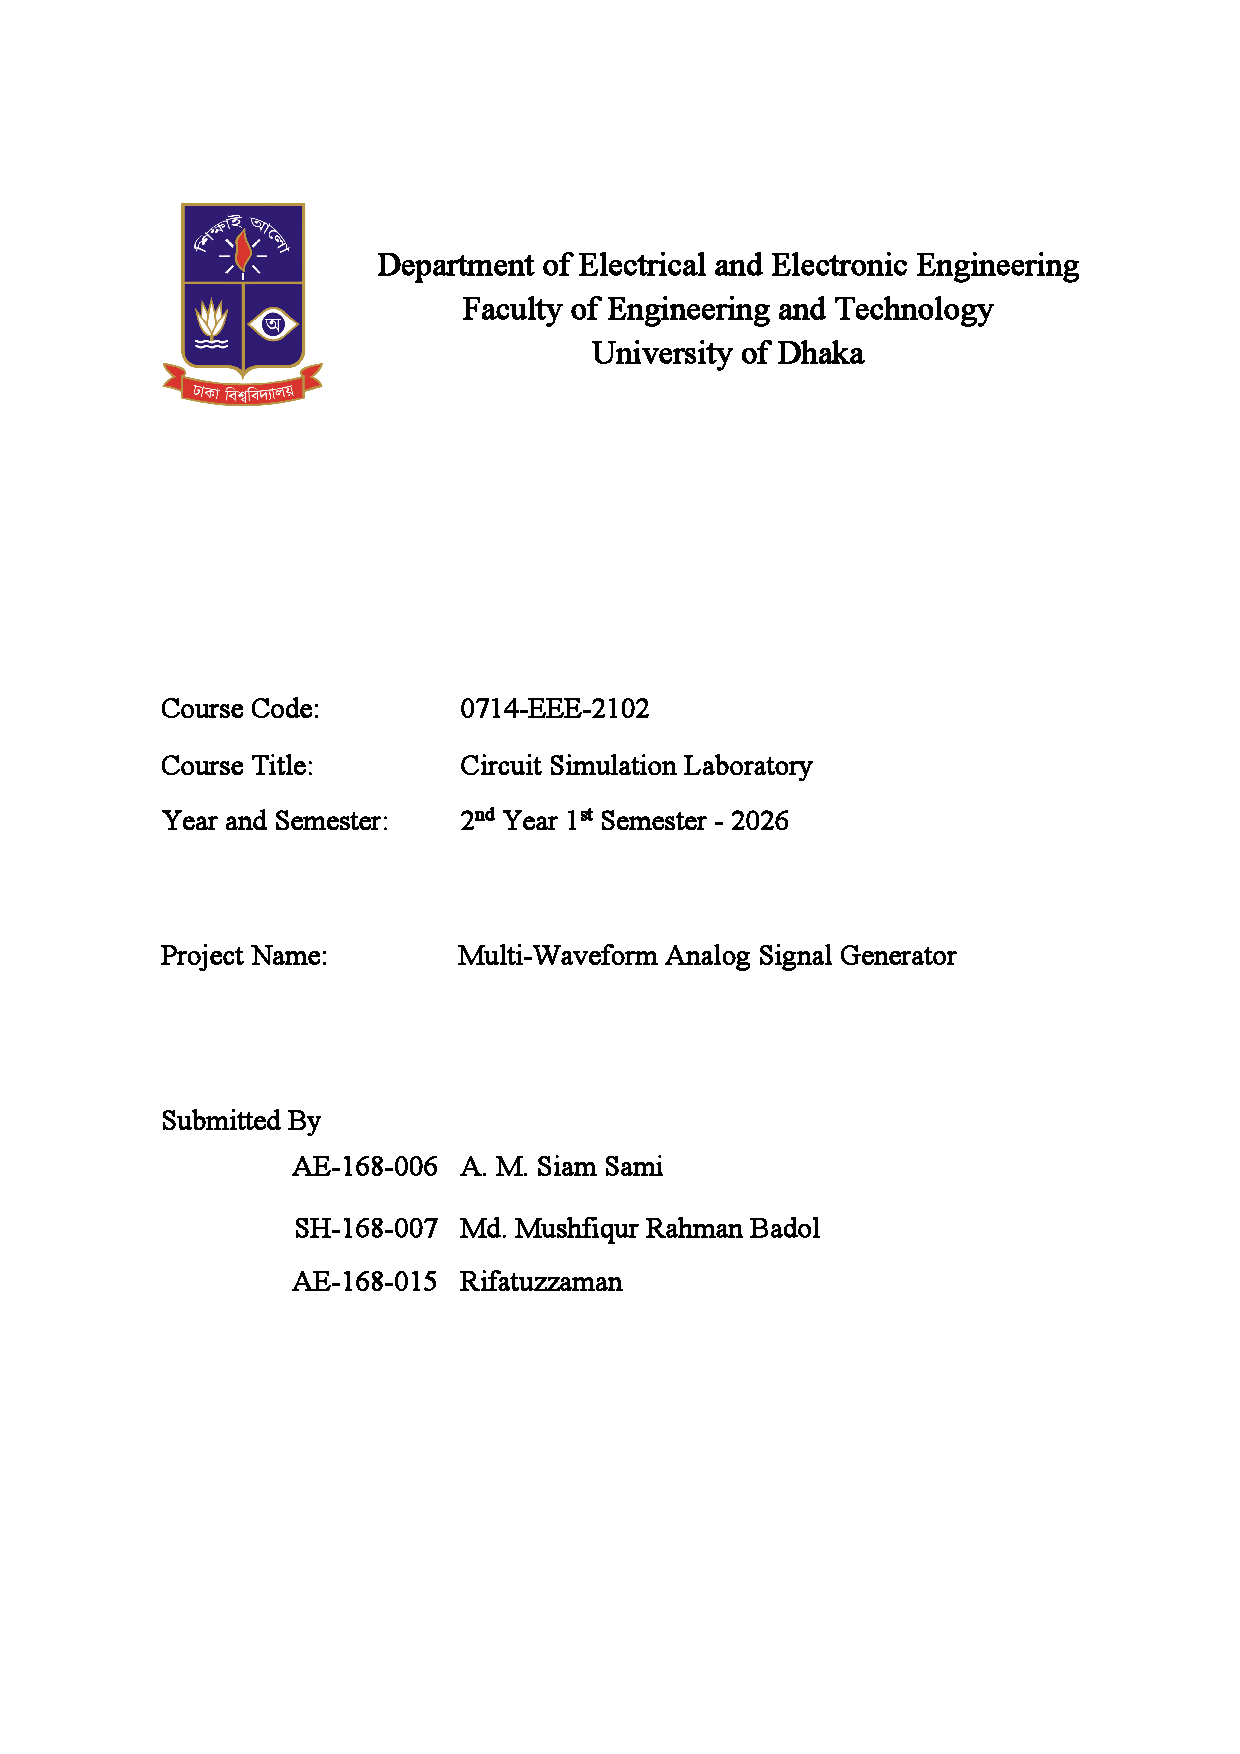
\includepdf[pages=1,pagecommand={\thispagestyle{empty}}]{../Cover Page of Project Report.pdf}

\tableofcontents
\newpage

% =====================================================================
\section{Project at a glance}
% =====================================================================
The project turns \textbf{mains AC into a regulated 12\,V rail} (Exp.\ 11, 04, 05) and then uses that rail to turn a \textbf{1\,kHz square wave} into a \textbf{triangle wave} (Exp.\ 01) and finally into a \textbf{sine wave} (Exp.\ 06), with BJT stages (Exp.\ 08, 09) providing gain and buffering. The numbers are hand calculations that I then checked in a circuit-level simulation with 2N2222 transistor models (Section~\ref{sec:sim}). That simulation is not Multisim, so repeat it in your lab simulator and replace $\beta$ and $V_D$ by the values you measured in Exp.~08 and Exp.~02.

\begin{figure}[H]
\centering
\resizebox{\textwidth}{!}{%
\begin{tikzpicture}[node distance=0.35cm]
% power chain
\node[pblk] (ac) at (0,0) {220\,V AC\\50\,Hz};
\node[pblk,right=0.45cm of ac] (tr) {Centre-tap\\transformer\\12-0-12\,V};
\node[pblk,right=0.45cm of tr] (rc) {Full-wave\\rectifier\\$D_1,D_2$};
\node[pblk,right=0.45cm of rc] (fl) {Filter\\$C_1=470\,\mu$F};
\node[pblk,right=0.45cm of fl] (zn) {Zener\\regulator\\12\,V};
\draw[arr] (ac)--(tr); \draw[arr] (tr)--(rc); \draw[arr] (rc)--(fl); \draw[arr] (fl)--(zn);
\node[font=\scriptsize,above=2pt of zn,xshift=1.7cm] {$\rightarrow$ +12\,V rail feeds $Q_1,Q_2,Q_3$ and the tap ladder};
% signal chain
\node[blk] (s1) at (0,-3.3) {Square\\source\\1\,kHz, $\pm5$\,V};
\node[blk,right=0.45cm of s1] (s2) {RC\\integrator\\510\,$\Omega$, 10\,$\mu$F};
\node[blk,right=0.45cm of s2] (s3) {$Q_1$ CE\\amplifier\\$A_v\approx-12.6$};
\node[blk,right=0.45cm of s3] (s4) {$Q_2$ emitter\\follower\\$A_v\approx0.99$};
\node[blk,right=0.45cm of s4] (s5) {Diode\\shaper\\4 diodes};
\node[blk,right=0.45cm of s5] (s6) {$Q_3$ emitter\\follower\\output};
\foreach \a/\b in {s1/s2,s2/s3,s3/s4,s4/s5,s5/s6} \draw[arr] (\a)--(\b);
% mini waveforms
\newcommand{\mini}[4]{\begin{tikzpicture}\begin{axis}[width=2.9cm,height=1.55cm,scale only axis,axis lines=left,ticks=none,
   ymin=#2,ymax=#3,xmin=0,xmax=2,domain=0:2,samples=300,no markers,thick,smooth]\addplot[#4]{#1};\end{axis}\end{tikzpicture}}
\node[below=0.15cm of s1] {\mini{5*sign(sin(360*x))}{-6.5}{6.5}{ctp1}};
\node[below=0.15cm of s2] {\mini{\TRI{x}}{-0.4}{0.4}{ctp2}};
\node[below=0.15cm of s3] {\mini{6-12.47*\TRI{x}}{2}{10}{ctp3}};
\node[below=0.15cm of s4] {\mini{6-12.3*\TRI{x}}{2}{10}{ctp3}};
\node[below=0.15cm of s5] {\mini{6+shp(-12.47*\TRI{x})}{3.5}{8.5}{ctp4}};
\node[below=0.15cm of s6] {\mini{0.99*shp(-12.47*\TRI{x})}{-3}{3}{ctp5}};
\node[font=\tiny,below=1.95cm of s1] {TP1};
\node[font=\tiny,below=1.95cm of s2] {TP2: 0.49\,V$_{pp}$};
\node[font=\tiny,below=1.95cm of s3] {$Q_1$ collector: 6.2\,V$_{pp}$};
\node[font=\tiny,below=1.95cm of s4] {TP3: 6.1\,V$_{pp}$};
\node[font=\tiny,below=1.95cm of s5] {TP4: 4\,V$_{pp}$};
\node[font=\tiny,below=1.95cm of s6] {TP5: 3.9\,V$_{pp}$};
\end{tikzpicture}}
\caption{System block diagram. The small plots show the waveform at the output of each signal-chain block (two periods, steady state, from the hand-calculation model of Section~\ref{sec:wave}).}
\label{fig:blocks}
\end{figure}

\subsection{Design targets}
\begin{center}
\small
\begin{tabularx}{\textwidth}{@{}lXl@{}}
\toprule
Item & Target & Experiments used \\
\midrule
DC adapter & 220\,V AC $\rightarrow$ 12\,V regulated, ripple $<$ 60\,mV$_{pp}$, 20\,mA max & 11, 04, 05 \\
Square wave & 1\,kHz, 10\,V$_{pp}$, 50\,\% duty (function generator) & --- \\
Triangle wave & linear to about 1--2\,\%, 6\,V$_{pp}$ after amplification & 01 \\
Sine wave & about 4\,V$_{pp}$ around a 6\,V level, THD below 5\,\% & 06 (V$_D$ from 02) \\
Amplification and buffering & $Q_1$ gain $\approx-12.6$, two emitter followers & 08, 09 \\
Optional DC restoration & negative clamp at the output & 07 \\
\bottomrule
\end{tabularx}
\end{center}

\subsection{Test points}
\begin{center}
\small
\begin{tabular}{@{}llll@{}}
\toprule
TP & Location & Waveform & Expected \\
\midrule
TP1 & source output & square & 10\,V$_{pp}$, 1\,kHz \\
TP2 & integrator node & triangle & $\approx$0.49\,V$_{pp}$ \\
TP3 & $Q_2$ emitter & amplified triangle & $\approx$6.1\,V$_{pp}$ around 6\,V (inverted) \\
TP4 & shaper node $X$ & shaped sine & $\approx$4\,V$_{pp}$ around 6\,V \\
TP5 & final output & sine & $\approx$3.8--4.0\,V$_{pp}$ \\
\bottomrule
\end{tabular}
\end{center}

% =====================================================================
\section{Workflow}
% =====================================================================
Build and verify \textbf{one stage at a time}. Do not connect the next stage until the current one meets its expected values; if it does not, fix it before moving on.

\begin{figure}[H]
\centering
\resizebox{\textwidth}{!}{%
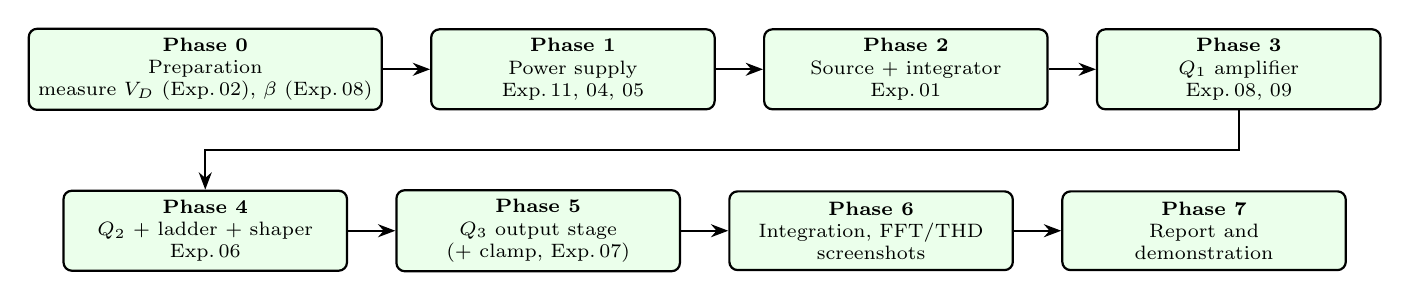
\begin{tikzpicture}
\node[ph] (p0) at (0,0) {\textbf{Phase 0}\\Preparation\\measure $V_D$ (Exp.\,02), $\beta$ (Exp.\,08)};
\node[ph,right=0.6cm of p0] (p1) {\textbf{Phase 1}\\Power supply\\Exp.\,11, 04, 05};
\node[ph,right=0.6cm of p1] (p2) {\textbf{Phase 2}\\Source + integrator\\Exp.\,01};
\node[ph,right=0.6cm of p2] (p3) {\textbf{Phase 3}\\$Q_1$ amplifier\\Exp.\,08, 09};
\node[ph,below=1.0cm of p0] (p4) {\textbf{Phase 4}\\$Q_2$ + ladder + shaper\\Exp.\,06};
\node[ph,right=0.6cm of p4] (p5) {\textbf{Phase 5}\\$Q_3$ output stage\\(+ clamp, Exp.\,07)};
\node[ph,right=0.6cm of p5] (p6) {\textbf{Phase 6}\\Integration, FFT/THD\\screenshots};
\node[ph,right=0.6cm of p6] (p7) {\textbf{Phase 7}\\Report and\\demonstration};
\draw[arr] (p0)--(p1); \draw[arr] (p1)--(p2); \draw[arr] (p2)--(p3);
\draw[arr] (p3.south) -- ++(0,-0.5) -| (p4.north);
\draw[arr] (p4)--(p5); \draw[arr] (p5)--(p6); \draw[arr] (p6)--(p7);
\end{tikzpicture}}
\caption{Build order. After every phase compare node voltages and waveforms with the expected values in Section~\ref{sec:expected} before continuing.}
\end{figure}

\begin{tabularx}{\textwidth}{@{}lX@{}}
\toprule
Phase & What to do and what to check \\
\midrule
0 & Read $V_D$ at about 1\,mA from your Exp.\,02 I-V curve and $\beta$ from Exp.\,08. Use them instead of 0.65\,V and 100. \\
1 & Build transformer, two diodes, 470\,$\mu$F and Zener with a 600\,$\Omega$ test load. Check: filter ripple $\approx$0.75\,V$_{pp}$, output 12\,V $\pm$0.3\,V, Zener current $>5$\,mA. \\
2 & 1\,kHz, $\pm5$\,V square into 510\,$\Omega$/10\,$\mu$F. Check: triangle of $\approx$0.49\,V$_{pp}$ at TP2. \\
3 & Check DC first ($V_B\approx1.8$\,V, $V_E\approx1.1$\,V, $V_C\approx6.9$\,V), then gain $\approx-12.6$ with $Q_2$ attached. \\
4 & Check ladder taps (4.90, 5.63, 6.37, 7.10\,V), then TP4 must look like a rounded sine. \\
5 & Check TP5 amplitude and shape with 10\,k$\Omega$ load; add the Exp.\,07 clamp as an optional extra. \\
6 & Run all stages together; capture the four scope channels; run Fourier analysis (1\,kHz fundamental, 9 harmonics). \\
7 & Write the report using Section~\ref{sec:report}; rehearse the 3--5 minute demonstration. \\
\bottomrule
\end{tabularx}

% =====================================================================
\section{Stage-by-stage design}
% =====================================================================
Notation: $f=1$\,kHz, $T=1$\,ms, $V_{CC}=12$\,V, $V_D=0.65$\,V, $V_T=25$\,mV. The hand calculations use $\beta=100$; the simulation with the real 2N2222 model ($\beta\approx256$) gives somewhat different DC levels (Section~\ref{sec:sim}), and the design still works.

% ---------------------------------------------------------------------
\subsection{Power supply: transformer, rectifier, filter, Zener (Exp.\ 11, 04, 05)}
% ---------------------------------------------------------------------
\begin{figure}[H]
\centering
\resizebox{\textwidth}{!}{\begin{circuitikz}[font=\scriptsize,line width=0.7pt]
\psuckt
\end{circuitikz}}
\caption{DC adapter. Markers a--d are the nodes whose waveforms are plotted in Fig.~\ref{fig:psuwave}. Marker b is the rectifier output with $C_1$ removed (Exp.\,04, no filter); with $C_1$ connected the same node gives waveform c.}
\end{figure}

\begin{figure}[H]
\centering
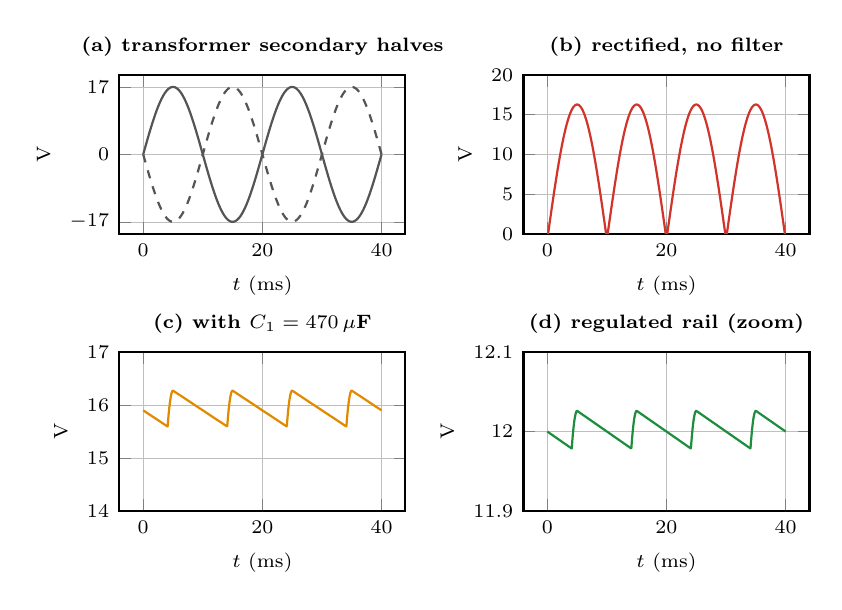
\begin{tikzpicture}
\begin{groupplot}[group style={group size=2 by 2,horizontal sep=1.5cm,vertical sep=1.5cm},wf,width=0.43\textwidth,height=3.6cm,
  domain=0:40,samples=900]
\nextgroupplot[title={(a) transformer secondary halves},ymin=-20,ymax=20,ytick={-16.97,0,16.97},yticklabels={$-17$,$0$,$17$},ylabel={V}]
\addplot[ctpa] {16.97*sin(18*x)};
\addplot[ctpa,dashed] {-16.97*sin(18*x)};
\nextgroupplot[title={(b) rectified, no filter},ymin=0,ymax=20,ylabel={V}]
\addplot[ctp2] {max(16.97*abs(sin(18*x))-0.7,0)};
\nextgroupplot[title={(c) with $C_1=470\,\mu$F},ymin=14,ymax=17,ylabel={V}]
\addplot[ctp3] {max(16.97*abs(sin(18*x))-0.7,16.27-0.0745*mod(x+5,10))};
\nextgroupplot[title={(d) regulated rail (zoom)},ymin=11.9,ymax=12.1,ytick={11.9,12,12.1},ylabel={V}]
\addplot[ctp5] {12+0.07*(max(16.97*abs(sin(18*x))-0.7,16.27-0.0745*mod(x+5,10))-15.9)};
\end{groupplot}
\end{tikzpicture}
\caption{Power-supply waveforms over two mains cycles (40\,ms). The ripple falls from 0.745\,V$_{pp}$ across $C_1$ to about 52\,mV$_{pp}$ after the Zener.}
\label{fig:psuwave}
\end{figure}

\begin{tcolorbox}[colback=blue!3,colframe=blue!40!black,title=Calculations,fonttitle=\small\bfseries,boxrule=0.4pt]
\small
\begin{align*}
V_m&=12\sqrt2=16.97\,\mathrm{V},\quad V_{peak}=16.97-0.7=16.27\,\mathrm{V},\quad \mathrm{PIV}=2V_m=33.9\,\mathrm{V}\ (\text{1N4007})\\
C_1&\ge\frac{I}{2fV_r}=\frac{35\,\mathrm{mA}}{2\cdot50\cdot1\,\mathrm{V}}=350\,\mu\mathrm F\;\Rightarrow\;470\,\mu\mathrm F,\qquad V_r=\frac{0.035}{100\cdot470\,\mu}=0.745\,\mathrm{V_{pp}}\\
V_{dc}&=16.27-\tfrac{0.745}{2}=15.9\,\mathrm V,\quad V_{min}=15.53\,\mathrm V,\quad r=\frac{V_r}{2\sqrt3V_{dc}}=1.35\,\%\\
R_S&\le\frac{V_{min}-V_Z}{I_{L(max)}+I_{Z(min)}}=\frac{15.53-12}{20+5\ \mathrm{mA}}=141\,\Omega\;\Rightarrow\;R_S=120\,\Omega\ (0.5\,\mathrm W)
\end{align*}
\begin{center}
\begin{tabular}{@{}lccl@{}}
\toprule
Condition & $I_{R_S}$ & $I_Z$ & Result \\
\midrule
Nominal (15.9\,V, 12\,mA load) & 32.5\,mA & 20.5\,mA & $P_Z=246$\,mW \\
Worst low (15.53\,V, 20\,mA load) & 29.4\,mA & 9.4\,mA & $>5$\,mA, OK \\
Worst high, no load (16.27\,V) & 35.6\,mA & 35.6\,mA & $P_Z=427$\,mW $<1$\,W, OK \\
\bottomrule
\end{tabular}
\end{center}
Output ripple $=0.745\cdot\frac{9}{120+9}\approx52$\,mV$_{pp}$ ($r_z\approx9\,\Omega$); load regulation $\approx8\,\mathrm{mA}\cdot9\,\Omega=72$\,mV (0.6\,\%).
\end{tcolorbox}

% ---------------------------------------------------------------------
\subsection{Square source and RC integrator (Exp.\ 01)}
% ---------------------------------------------------------------------
\begin{figure}[H]
\centering
\resizebox{0.78\textwidth}{!}{\begin{circuitikz}[font=\scriptsize,line width=0.7pt]
\integckt
\node[font=\tiny,above] at ($(iout)+(0.2,0.0)$) {to $Q_1$};
\end{circuitikz}}
\caption{Square source and RC integrator. The integrator sees $Q_1$'s input impedance $Z_{in1}=5.2\,\mathrm{k}\Omega$ in parallel with $C_{int}$.}
\end{figure}

\begin{figure}[H]
\centering
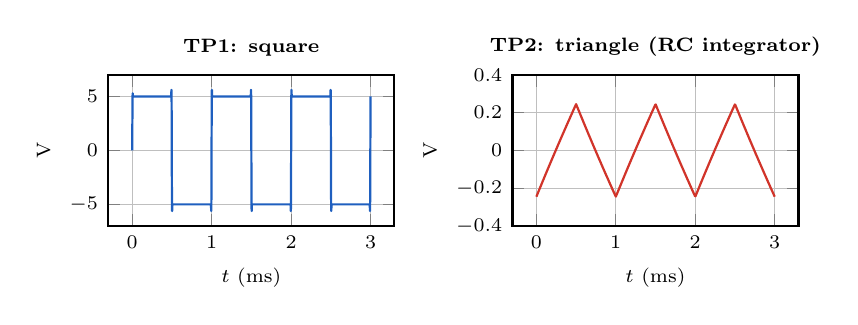
\begin{tikzpicture}
\begin{groupplot}[group style={group size=2 by 1,horizontal sep=1.5cm},wf,width=0.43\textwidth,domain=0:3]
\nextgroupplot[title={TP1: square},ymin=-7,ymax=7,xlabel={$t$ (ms)},ylabel={V}]
\addplot[ctp1] {5*sign(sin(360*x))};
\nextgroupplot[title={TP2: triangle (RC integrator)},ymin=-0.4,ymax=0.4,ylabel={V}]
\addplot[ctp2] {\TRI{x}};
\end{groupplot}
\end{tikzpicture}
\caption{The square wave is integrated into a triangle of $0.49\,\mathrm{V_{pp}}$. The slight exponential curvature is the 1.4\,\% non-linearity of the RC charging curve.}
\end{figure}

\begin{tcolorbox}[colback=blue!3,colframe=blue!40!black,title=Calculations,fonttitle=\small\bfseries,boxrule=0.4pt]
\small
For $RC\gg T/2$ the capacitor charges almost linearly, so $V_{pp}=\dfrac{A\,T}{2RC}$. Target $V_{pp}\approx0.48$\,V (so that $Q_1$ delivers $\pm3$\,V) gives $RC\approx5.2$\,ms $\Rightarrow$ $R=510\,\Omega$, $C=10\,\mu$F ($RC=5.1$\,ms $\approx5T$).
\begin{align*}
V_{th}&=5\cdot\frac{5200}{510+5200}=4.55\,\mathrm V,\quad R_{th}=510\parallel5200=464\,\Omega,\quad \tau=R_{th}C=4.64\,\mathrm{ms}\\
V_{pp}&=\frac{V_{th}\,T}{2\tau}=\frac{4.55\cdot1\,\mathrm{ms}}{2\cdot4.64\,\mathrm{ms}}=0.49\,\mathrm{V_{pp}}\qquad(\text{loading cancels: }V_{th}/R_{th}=A/R)\\
\text{non-linearity}&\approx\frac{(V_{th}+V_p)(T/2\tau)^2}{8\,V_{pp}}=\frac{4.8\cdot0.0116/8}{0.49}\approx1.4\,\%
\end{align*}
\textbf{Important:} the triangle amplitude is proportional to $1/f$. Keep the source at 1\,kHz, or rescale $R$ so that $RC\approx5T$ if you change the frequency.
\end{tcolorbox}

% ---------------------------------------------------------------------
\subsection{$Q_1$: common-emitter amplifier (Exp.\ 08, 09)}
% ---------------------------------------------------------------------
\begin{figure}[H]
\centering
\resizebox{0.86\textwidth}{!}{\begin{circuitikz}[font=\scriptsize,line width=0.7pt]
\qoneckt
\node[font=\tiny,right] at ($(q1out)+(0.05,0)$) {to $Q_2$};
\end{circuitikz}}
\caption{$Q_1$ common-emitter amplifier with voltage-divider bias and a partly bypassed emitter resistor (gain set by $R_{E1}$).}
\end{figure}

\begin{figure}[H]
\centering
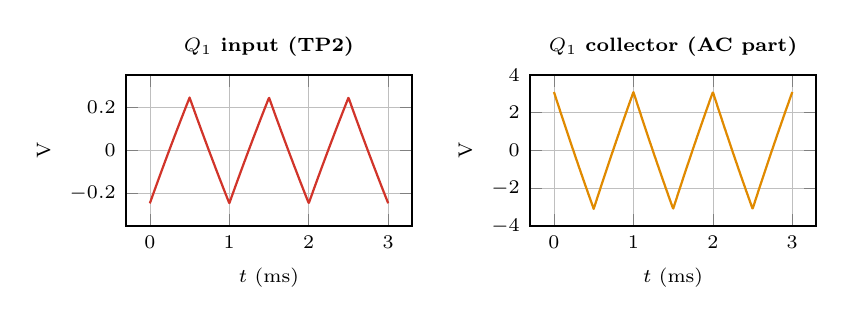
\begin{tikzpicture}
\begin{groupplot}[group style={group size=2 by 1,horizontal sep=1.5cm},wf,width=0.43\textwidth,domain=0:3]
\nextgroupplot[title={$Q_1$ input (TP2)},ymin=-0.35,ymax=0.35,ylabel={V}]
\addplot[ctp2] {\TRI{x}};
\nextgroupplot[title={$Q_1$ collector (AC part)},ymin=-4,ymax=4,ylabel={V}]
\addplot[ctp3] {-12.63*\TRI{x}};
\end{groupplot}
\end{tikzpicture}
\caption{$Q_1$ amplifies the 0.49\,V$_{pp}$ triangle by $-12.6$ to 6.2\,V$_{pp}$. The minus sign means the output is 180$^\circ$ out of phase with the input.}
\end{figure}

\begin{tcolorbox}[colback=blue!3,colframe=blue!40!black,title=Calculations,fonttitle=\small\bfseries,boxrule=0.4pt]
\small
$R_{C1}=2.7\,\mathrm{k}\Omega$, $R_{E1}=150\,\Omega$ (unbypassed), $R_{E2}=430\,\Omega$ (bypassed), $R_{B1}=47\,\mathrm{k}\Omega$, $R_{B2}=9.1\,\mathrm{k}\Omega$.
\begin{align*}
V_{TH}&=12\cdot\tfrac{9.1}{56.1}=1.95\,\mathrm V,\quad R_{TH}=47\parallel9.1=7.62\,\mathrm{k}\Omega\\
I_E&=\frac{V_{TH}-0.7}{R_E+R_{TH}/(\beta+1)}=\frac{1.246}{580+75.5}=1.90\,\mathrm{mA},\quad V_E=1.10\,\mathrm V,\ V_B=1.80\,\mathrm V,\ V_C=12-1.88\cdot2.7=6.92\,\mathrm V\\
r_e&=\frac{25\,\mathrm{mV}}{1.90\,\mathrm{mA}}=13.1\,\Omega,\quad Z_{in1}=R_{B1}\parallel R_{B2}\parallel\beta(r_e+R_{E1})=7.62\parallel16.3=5.2\,\mathrm{k}\Omega\\
A_{v1}&=-\frac{R_{C1}\parallel Z_{in2}}{r_e+R_{E1}}=-\frac{2.7\parallel8.7}{0.1631}=-\frac{2.06\,\mathrm{k}}{163.1\,\Omega}=-12.6\\
\text{output}&=0.49\cdot12.6=6.2\,\mathrm{V_{pp}}\ (\pm3.1\,\mathrm V);\quad\text{headroom }I_C\,r_{ac}=1.88\cdot2.06=\pm3.9\,\mathrm V\ \checkmark
\end{align*}
Coupling: $C_4$ gives $f_c\approx3$\,Hz, $C_5$ about 1.4\,Hz, $C_E=100\,\mu$F about 10\,Hz, all far below 1\,kHz.
\end{tcolorbox}

% ---------------------------------------------------------------------
\subsection{$Q_2$: emitter-follower buffer}
% ---------------------------------------------------------------------
\begin{figure}[H]
\centering
\resizebox{0.62\textwidth}{!}{\begin{circuitikz}[font=\scriptsize,line width=0.7pt]
\qtwockt
\node[font=\tiny,above] at ($(q2in)+(0.0,0.0)$) {from $Q_1$};
\tpmark[right]{q2out}{TP3}
\end{circuitikz}}
\caption{$Q_2$ emitter follower. Its emitter sits at about 6\,V DC, which becomes the common centre level of the shaper.}
\end{figure}

\begin{figure}[H]
\centering
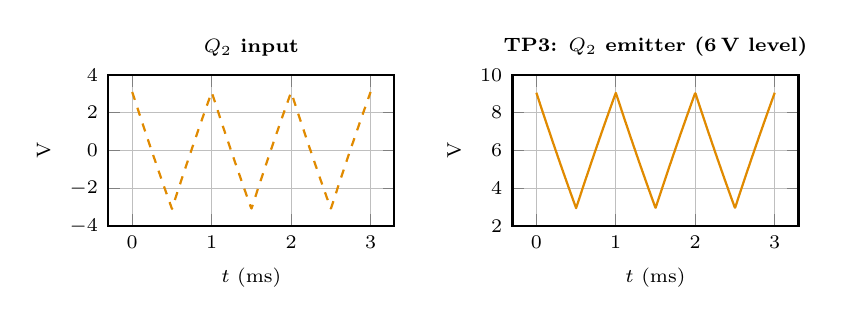
\begin{tikzpicture}
\begin{groupplot}[group style={group size=2 by 1,horizontal sep=1.5cm},wf,width=0.43\textwidth,domain=0:3]
\nextgroupplot[title={$Q_2$ input},ymin=-4,ymax=4,ylabel={V}]
\addplot[ctp3,dashed] {-12.63*\TRI{x}};
\nextgroupplot[title={TP3: $Q_2$ emitter (6\,V level)},ymin=2,ymax=10,ylabel={V}]
\addplot[ctp3] {6-12.47*\TRI{x}};
\end{groupplot}
\end{tikzpicture}
\caption{The follower reproduces the triangle with gain 0.99 and shifts it to a 6\,V DC level. Low output impedance now isolates $Q_1$ from the shaper.}
\end{figure}

\begin{tcolorbox}[colback=blue!3,colframe=blue!40!black,title=Calculations,fonttitle=\small\bfseries,boxrule=0.4pt]
\small
\begin{align*}
V_{TH}&=12\cdot\tfrac{22}{38}=6.95\,\mathrm V,\ R_{TH}=16\parallel22=9.26\,\mathrm{k}\Omega,\quad I_E=\frac{6.95-0.7}{2000+9260/101}=2.99\,\mathrm{mA},\quad V_E=5.97\approx6.0\,\mathrm V\\
r_e&=8.4\,\Omega,\quad A_v\approx\frac{r_{ac}}{r_e+r_{ac}}\approx0.99,\quad Z_{in2}=R_{B3}\parallel R_{B4}\parallel\beta(r_e+r_{ac})=9.26\parallel151=8.7\,\mathrm{k}\Omega\\
Z_{out}&\approx r_e+\frac{R_{C1}\parallel R_{B3}\parallel R_{B4}}{\beta}=8.4+\frac{2.09\,\mathrm k}{100}\approx29\,\Omega\ \ll R_{SH}=2.2\,\mathrm{k}\Omega\ \checkmark
\end{align*}
\end{tcolorbox}

% ---------------------------------------------------------------------
\subsection{Diode shaper: triangle to sine (Exp.\ 06)}
% ---------------------------------------------------------------------
The shaper is a \textbf{piecewise-linear sine approximation}. A series resistor $R_{SH}$ feeds node $X$. Four shunt branches (resistor + diode + bias tap) turn on one after another as the triangle approaches its peaks. Each branch that turns on lowers the slope, so the pointed triangle tip is rounded into a sine. All taps are referenced to the 6\,V centre level, so a single 12\,V rail is enough. The shaper input is \textbf{AC coupled} ($C_{sh}$) and node $X$ is tied to the ladder centre (6.00\,V) through $R_{ref}$. This was added after the first simulation showed that $Q_2$'s emitter sits at 6.1--6.25\,V with real 2N2222 gain, while the taps are centred on 6.0\,V; the mismatch made the shaping asymmetric (6\,\% THD, mostly second harmonic). With the coupling capacitor the shaper no longer depends on $\beta$.

\begin{figure}[H]
\centering
\resizebox{\textwidth}{!}{\begin{circuitikz}[font=\scriptsize,line width=0.7pt]
\shapckt
\begin{scope}[shift={(15.4,-0.2)}]
\ladckt
\end{scope}
\node[font=\scriptsize,align=center] at (15.4,-3.2) {bias ladder (each tap bypassed\\with $10\,\mu$F to ground)};
\end{circuitikz}}
\caption{Shaper (left) and its bias ladder (right). The yellow boxes are the same four tap voltages in both drawings: the ladder produces them, the branches use them. Upper branches conduct when $V_X$ rises above tap + 0.65\,V; lower branches when it falls below tap $-$ 0.65\,V.}
\label{fig:shaper}
\end{figure}

\begin{figure}[H]
\centering
\begin{tikzpicture}
\begin{groupplot}[group style={group size=2 by 1,horizontal sep=1.6cm},wf,width=0.43\textwidth,height=4.4cm]
\nextgroupplot[title={Shaper transfer characteristic},xlabel={input relative to 6\,V (V)},ylabel={$V_X$ rel.\ to 6\,V (V)},
  domain=-3.4:3.4,samples=400,xmin=-3.4,xmax=3.4,ymin=-2.4,ymax=2.4,legend style={font=\tiny,at={(0.03,0.97)},anchor=north west}]
\addplot[gray,dashed] {0.9442*x};
\addplot[ctp4] {shp(x)};
\addplot[ctp5,dotted,domain=-3.056:3.056] {1.97*sin(90*x/3.056)};
\legend{no diodes,with shaper,ideal sine}
\nextgroupplot[title={TP3 $\rightarrow$ TP4 (one period)},domain=0:2,xmin=0,xmax=2,ymin=-4,ymax=4,
  legend style={font=\tiny,at={(0.03,0.97)},anchor=north west},ylabel={V relative to 6\,V}]
\addplot[ctp3] {-12.47*\TRI{x}};
\addplot[ctp4] {shp(-12.47*\TRI{x})};
\addplot[black,dotted] {1.97*cos(360*x)};
\legend{TP3 triangle,TP4 shaped,ideal sine}
\end{groupplot}
\end{tikzpicture}
\caption{Left: the slope falls from 0.94 to 0.71 to 0.26 as branches turn on, tracking the ideal sine. Right: the pointed triangle (orange) becomes the shaped wave (purple), close to the ideal sine (dotted).}
\end{figure}

\begin{tcolorbox}[colback=blue!3,colframe=blue!40!black,title=Calculations,fonttitle=\small\bfseries,boxrule=0.4pt]
\small
\textbf{1. Break points.} Split each quarter cycle at $30^\circ$ and $60^\circ$. A triangle is linear in angle, so for a sine of peak $V_o$:
\begin{center}
\begin{tabular}{@{}cccc@{}}
\toprule
Segment & Angle & Sine rise & Relative slope \\
\midrule
1 & $0^\circ$--$30^\circ$ & $0.500V_o$ & 1.000 \\
2 & $30^\circ$--$60^\circ$ & $0.366V_o$ & 0.732 \\
3 & $60^\circ$--$90^\circ$ & $0.134V_o$ & 0.268 \\
\bottomrule
\end{tabular}
\end{center}
With segment 1 untouched, $V_o=2.0$\,V and the break points are $V_X=1.00$\,V and $1.73$\,V above the 6\,V centre.

\textbf{2. Taps} (turn-on at tap $+V_D$): tap$_1=1.00-0.65=0.35$\,V and tap$_2=1.73-0.65=1.08$\,V above centre; the lower taps mirror them.

\textbf{3. Resistors} with $R_{SH}=2.2\,\mathrm{k}\Omega$, using slope $=R_p/(R_{SH}+R_p)$:
\[
R_{P1}=\frac{0.732}{0.268}R_{SH}=6.0\,\mathrm{k}\Omega\Rightarrow6.2\,\mathrm{k}\Omega,\qquad
\frac1{R_{P2}}=\frac{1}{0.366R_{SH}}-\frac1{R_{P1}}\Rightarrow R_{P2}\approx925\,\Omega\Rightarrow910\,\Omega
\]
\textbf{4. Ladder} $1.2\,\mathrm k+180+91+91+180\,\Omega+1.2\,\mathrm k=2.94\,\mathrm{k}\Omega$, $I=4.08$\,mA, taps $4.90,\ 5.63,\ 6.37,\ 7.10$\,V and an explicit centre node at 6.00\,V (the 180\,$\Omega$ middle resistor is split in two). $C_{sh}=10\,\mu$F and $R_{ref}=100\,\mathrm{k}\Omega$ then set node $X$ to 6.00\,V DC.

\textbf{5. Loaded slopes} (including $Z_{in3}=37.7\,\mathrm k\Omega$ and $Z_{out,Q_2}=29\,\Omega$):
\begin{center}
\begin{tabular}{@{}lccc@{}}
\toprule
Segment & Slope $V_X/V_{in}$ & Relative to segment 1 & Target \\
\midrule
1 (no diode) & 0.944 & 1.000 & 1.000 \\
2 (upper branch 1 on) & 0.705 & 0.747 & 0.732 \\
3 (both on) & 0.259 & 0.274 & 0.268 \\
\bottomrule
\end{tabular}
\end{center}
Break points in terms of the input: 1.08\,V and 2.12\,V. With a $\pm3.06$\,V triangle, node $X$ peaks at $\pm1.99$\,V ($\approx4$\,V$_{pp}$).
\end{tcolorbox}

\begin{center}
\small
\begin{tabularx}{\textwidth}{@{}llllX@{}}
\toprule
Branch & Resistor & Diode (anode $\rightarrow$ cathode) & Tap & Turns on when \\
\midrule
U1 & $R_{P1}$ 6.2\,k$\Omega$ & toward $X$ $\rightarrow$ tap & 6.37\,V & $V_X>7.02$\,V \\
U2 & $R_{P2}$ 910\,$\Omega$ & toward $X$ $\rightarrow$ tap & 7.10\,V & $V_X>7.75$\,V \\
L1 & $R_{P1}$ 6.2\,k$\Omega$ & tap $\rightarrow$ toward $X$ & 5.63\,V & $V_X<4.98$\,V \\
L2 & $R_{P2}$ 910\,$\Omega$ & tap $\rightarrow$ toward $X$ & 4.90\,V & $V_X<4.25$\,V \\
\bottomrule
\end{tabularx}
\end{center}

% ---------------------------------------------------------------------
\subsection{$Q_3$: output emitter follower (and optional Exp.\ 07 clamp)}
% ---------------------------------------------------------------------
\begin{figure}[H]
\centering
\resizebox{0.9\textwidth}{!}{\begin{circuitikz}[font=\scriptsize,line width=0.7pt]
\qthreeckt
\node[font=\tiny,above] at ($(q3in)+(0.0,0.0)$) {from node $X$};
\end{circuitikz}}
\caption{$Q_3$ output stage. The high input impedance (37.7\,k$\Omega$) keeps the shaper slopes unchanged. The dashed diode $D_7$ is the optional negative clamp.}
\end{figure}

\begin{figure}[H]
\centering
\begin{tikzpicture}
\begin{groupplot}[group style={group size=2 by 1,horizontal sep=1.6cm},wf,width=0.43\textwidth,domain=0:2,xmin=0,xmax=2]
\nextgroupplot[title={TP5: final sine (AC coupled)},ymin=-3,ymax=3,ylabel={V}]
\addplot[ctp5] {0.99*shp(-12.47*\TRI{x})};
\nextgroupplot[title={Optional Exp.\,07 clamp output},ymin=-1.5,ymax=3.5,ylabel={V}]
\addplot[ctp5,dashed] {0.99*shp(-12.47*\TRI{x})};
\addplot[ctp5] {0.99*shp(-12.47*\TRI{x})+1.27};
\end{groupplot}
\end{tikzpicture}
\caption{Left: the output sine, $\pm1.97$\,V. Right: with the optional clamp $D_7$ the negative peaks are held at about $-0.7$\,V, so the whole sine rides on a DC level (dashed = unclamped, solid = clamped, not to scale of the diode knee).}
\end{figure}

\begin{tcolorbox}[colback=blue!3,colframe=blue!40!black,title=Calculations,fonttitle=\small\bfseries,boxrule=0.4pt]
\small
\begin{align*}
V_{TH}&=6.0\,\mathrm V,\ R_{TH}=50\,\mathrm{k}\Omega,\quad I_E=\frac{6.0-0.7}{1800+50000/101}=2.31\,\mathrm{mA},\ V_E=4.16\,\mathrm V,\ V_{CE}=7.84\,\mathrm V\\
r_e&=10.8\,\Omega,\ r_{ac}=1.8\parallel10=1.525\,\mathrm{k}\Omega,\quad Z_{in3}=50\parallel\beta(r_e+r_{ac})=50\parallel153.6=37.7\,\mathrm{k}\Omega\\
A_v&\approx0.99,\quad Z_{out}\approx31\,\Omega,\quad V_{out}\approx0.99\times1.99\approx1.97\,\mathrm V\ \text{peak}\ (3.9\,\mathrm{V_{pp}}),\quad f_{c,out}\approx\frac{1}{2\pi\cdot10\,\mathrm k\cdot10\,\mu}=1.6\,\mathrm{Hz}
\end{align*}
Clamp: $R_{Load}C_{out}=100$\,ms $\gg T$, so $D_7$ (anode to ground, cathode to the output) clamps the negative peak at $\approx-0.7$\,V and the sine runs from about $-0.7$\,V to $+3.2$\,V.
\end{tcolorbox}

\begin{landscape}
% =====================================================================
\section{Complete signal-chain schematic}
% =====================================================================
Figure~\ref{fig:full} joins the five signal stages. The +12\,V symbols are all the same rail from the power supply (Section~3.1), and every ground symbol is the common ground.


\begin{figure}[H]
\centering
\resizebox{0.97\linewidth}{!}{\begin{circuitikz}[font=\scriptsize,line width=0.7pt]
\begin{scope}[shift={(0,0)}]\integckt\end{scope}
\begin{scope}[shift={(5.2,0)}]\qoneckt\end{scope}
\draw (iout) -- (q1in);
\begin{scope}[shift={(13.0,0)}]\qtwockt\end{scope}
\draw (q1out) |- (q2in);
\begin{scope}[shift={(17.0,-1.0)}]\shapckt\end{scope}
\draw (q2out) -| (shin);
\begin{scope}[shift={(30.0,-1.0)}]\qthreeckt\end{scope}
\draw (shout) -- ++(0.5,0) |- (q3in);
\node[tap] at ($(shin)+(2.0,5.6)$) {taps from ladder (Fig.~\ref{fig:shaper})};
\tpmark[above right]{q2out}{TP3}
\end{circuitikz}}
\caption{Complete signal chain: square source $\rightarrow$ RC integrator $\rightarrow$ $Q_1$ $\rightarrow$ $Q_2$ $\rightarrow$ diode shaper $\rightarrow$ $Q_3$ $\rightarrow$ output. Test points TP1--TP5 are marked in red.}
\label{fig:full}
\end{figure}
\end{landscape}

% =====================================================================
\section{Waveform evolution through the circuit}
\label{sec:wave}
% =====================================================================
\begin{figure}[H]
\centering
\begin{tikzpicture}
\begin{groupplot}[group style={group size=1 by 5,vertical sep=0.55cm,xlabels at=edge bottom,xticklabels at=edge bottom},
  wf,width=0.82\textwidth,height=3.0cm,domain=0:3,samples=900,xmin=0,xmax=3,
  title style={font=\scriptsize\bfseries,yshift=-2pt,anchor=south west,at={(0.01,0.88)},fill=white,inner sep=1pt}]
\nextgroupplot[title={TP1: square source, $\pm5$ V},ymin=-7,ymax=7,ylabel={V},ytick={-5,0,5}]
\addplot[ctp1] {5*sign(sin(360*x))};
\nextgroupplot[title={TP2: triangle after RC integrator, 0.49 V$_{pp}$},ymin=-0.4,ymax=0.4,ylabel={V},ytick={-0.25,0,0.25}]
\addplot[ctp2] {\TRI{x}};
\nextgroupplot[title={TP3: after $Q_1$ and $Q_2$, 6.1 V$_{pp}$ on a 6 V level (inverted)},ymin=1,ymax=11,ylabel={V},ytick={3,6,9}]
\addplot[ctp3] {6-12.47*\TRI{x}};
\nextgroupplot[title={TP4: after diode shaper, about 4 V$_{pp}$ on a 6 V level},ymin=2,ymax=10,ylabel={V},ytick={4,6,8}]
\addplot[ctp4] {6+shp(-12.47*\TRI{x})};
\nextgroupplot[title={TP5: final output, 3.9 V$_{pp}$ (AC coupled)},ymin=-3,ymax=3,ylabel={V},ytick={-2,0,2},xlabel={$t$ (ms)}]
\addplot[ctp5] {0.99*shp(-12.47*\TRI{x})};
\end{groupplot}
\end{tikzpicture}
\caption{All test points on the same time axis (three 1\,ms periods). Read top to bottom: square, triangle, amplified triangle, shaped wave, final sine. The final sine is 180$^\circ$ out of phase with the square wave because $Q_1$ inverts.}
\end{figure}

\begin{figure}[H]
\centering
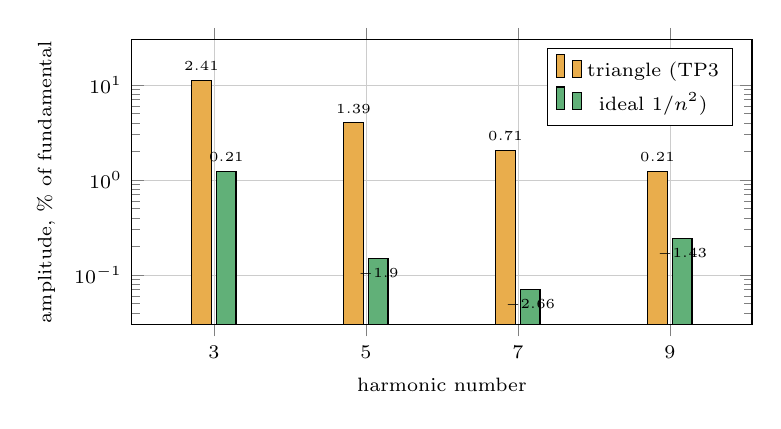
\begin{tikzpicture}
\begin{axis}[width=0.78\textwidth,height=5.2cm,ybar,bar width=7pt,ymode=log,log origin=infty,ymin=0.03,ymax=30,
  xtick={3,5,7,9},xlabel={harmonic number},ylabel={amplitude, \% of fundamental},grid=major,
  grid style={line width=.2pt,draw=gray!40},tick label style={font=\scriptsize},label style={font=\scriptsize},
  legend style={font=\scriptsize,at={(0.97,0.97)},anchor=north east},enlarge x limits=0.18,
  nodes near coords,every node near coord/.append style={font=\tiny,/pgf/number format/.cd,fixed,precision=2}]
\addplot[fill=ctp3!70] coordinates {(3,11.11) (5,4.00) (7,2.04) (9,1.23)};
\addplot[fill=ctp5!70] coordinates {(3,1.23) (5,0.15) (7,0.07) (9,0.24)};
\legend{triangle (TP3, ideal $1/n^2$),shaped sine (TP5, model)}
\end{axis}
\end{tikzpicture}
\caption{Harmonic content before and after the shaper. The third harmonic falls from 11.1\,\% to 1.2\,\%; the model THD of the final output is about 1.6\,\% (ideal 0.65\,V diodes). Real diodes have a soft knee; the circuit-level simulation of Section~\ref{sec:sim} gives 2.0\,\%.}
\end{figure}

% =====================================================================
\section{Supply current budget and bill of materials}
% =====================================================================
\begin{center}
\small
\begin{tabular}{@{}lr@{}}
\toprule
Block & Current \\
\midrule
$Q_1$ ($I_C$ + divider) & $1.88+0.21\approx2.1$\,mA \\
$Q_2$ ($I_E$ + divider) & $2.99+0.32\approx3.3$\,mA \\
$Q_3$ ($I_E$ + divider) & $2.31+0.06\approx2.4$\,mA \\
Bias ladder & 4.1\,mA \\
\midrule
\textbf{Total} & \textbf{$\approx$11.9\,mA (design limit 20\,mA)} \\
\bottomrule
\end{tabular}
\end{center}

\begin{center}
\small
\begin{tabularx}{\textwidth}{@{}llX@{}}
\toprule
Ref & Part & Value \\
\midrule
T1 & Transformer & 220\,V : 12-0-12\,V (ideal; ratio 9.17 over the full secondary) \\
$D_1,D_2$ & Rectifier diodes & 1N4007 \\
$C_1$, $C_2$ & Filter, rail decoupling & 470\,$\mu$F/25\,V, 100\,$\mu$F \\
$R_S$, $D_Z$ & Zener regulator & 120\,$\Omega$ 0.5\,W, 12\,V 1\,W (1N4742A) \\
$V_1$ & Function generator & 1\,kHz, 10\,V$_{pp}$ square, 0 offset \\
$R_{int}$, $C_{int}$ & Integrator & 510\,$\Omega$, 10\,$\mu$F \\
$Q_1,Q_2,Q_3$ & NPN transistors & 2N2222 (lab part) \\
$R_{B1},R_{B2},R_{C1}$ & $Q_1$ bias, collector & 47\,k$\Omega$, 9.1\,k$\Omega$, 2.7\,k$\Omega$ \\
$R_{E1},R_{E2},C_E$ & $Q_1$ emitter & 150\,$\Omega$, 430\,$\Omega$, 100\,$\mu$F \\
$C_4,C_5$ & $Q_1$ coupling & 10\,$\mu$F each \\
$R_{B3},R_{B4},R_{E3}$ & $Q_2$ & 16\,k$\Omega$, 22\,k$\Omega$, 2\,k$\Omega$ \\
$R_{SH}$, $C_{sh}$, $R_{ref}$ & Shaper series resistor, input coupling, centre reference & 2.2\,k$\Omega$, 10\,$\mu$F, 100\,k$\Omega$ \\
$R_{P1}$ (2), $R_{P2}$ (2) & Branch resistors & 6.2\,k$\Omega$, 910\,$\Omega$ \\
$D_3$--$D_6$ & Shaper diodes & 1N4148 \\
$R_{T1}$--$R_{T5}$ & Tap ladder ($R_{T3}$ split into $R_{T3a}$, $R_{T3b}$) & 1.2\,k, 180, 91, 91, 180, 1.2\,k$\Omega$ \\
Tap capacitors (5) & Bypass (four taps and centre) & 10\,$\mu$F each \\
$C_{10}$ & Coupling into $Q_3$ & 10\,$\mu$F \\
$R_{B5},R_{B6},R_{E4}$ & $Q_3$ & 100\,k$\Omega$, 100\,k$\Omega$, 1.8\,k$\Omega$ \\
$C_{out}$, $R_{Load}$ & Output & 10\,$\mu$F, 10\,k$\Omega$ \\
$D_7$ (optional) & Output clamp & 1N4148 \\
\bottomrule
\end{tabularx}
\end{center}


% =====================================================================
\section{Circuit-level simulation with 2N2222 models}
\label{sec:sim}
% =====================================================================
The hand model uses $\beta=100$ and ideal 0.65\,V diodes. To check the design with realistic devices, I simulated the complete circuit (power supply and signal chain) in a SPICE-style transient solver (modified nodal analysis, Newton iteration, 5\,$\mu$s step; junction capacitances are neglected, which is harmless at 1\,kHz). Device parameters are standard SPICE values:
\begin{center}
\small
\begin{tabular}{@{}ll@{}}
\toprule
Device & Parameters used \\
\midrule
2N2222 & $I_S=14.34$\,fA, $\beta_F=255.9$, $\beta_R=6.09$, $V_{AF}=74$\,V, $N_E=1.307$, $I_{SE}=14.34$\,fA, $r_b=10\,\Omega$ \\
1N4148 (shaper) & $I_S=2.52$\,nA, $N=1.752$, $R_S=0.568\,\Omega$ \\
1N4007 (rectifier) & $I_S=76.9$\,nA, $N=1.45$, $R_S=0.034\,\Omega$ \\
Zener 12\,V & $r_z\approx9\,\Omega$ at 20\,mA \\
Transformer & ideal 12-0-12\,V rms, 50\,Hz \\
\bottomrule
\end{tabular}
\end{center}
\textbf{Settling matters.} Because of the 10\,$\mu$F coupling capacitors, the waveform needs several hundred milliseconds to settle completely. The results below are from the settled state (0.6\,s run). Early in the run (first 30\,ms) the measured THD is much higher and misleading.

\subsection{Power supply}
\begin{figure}[H]
\centering
\begin{tikzpicture}
\begin{groupplot}[group style={group size=2 by 1,horizontal sep=1.5cm},wf,width=0.43\textwidth,xmin=0,xmax=40,samples=1000]
\nextgroupplot[title={Filter capacitor voltage},ymin=15.5,ymax=16.7,ylabel={V}]
\addplot[ctp3] table[x=t,y=dc]{psudata.dat};
\nextgroupplot[title={Regulated 12\,V rail},ymin=11.95,ymax=12.05,ylabel={V},ytick={11.95,12,12.05}]
\addplot[ctp5] table[x=t,y=vcc]{psudata.dat};
\end{groupplot}
\end{tikzpicture}
\caption{Simulated supply with the signal chain connected as its load (two mains cycles). The filter ripple is 0.64\,V$_{pp}$ around 16.1\,V and the rail is 12.01\,V with 37\,mV$_{pp}$ of ripple.}
\end{figure}

\subsection{Signal chain}
\begin{figure}[H]
\centering
\begin{tikzpicture}
\begin{groupplot}[group style={group size=1 by 5,vertical sep=0.55cm,xlabels at=edge bottom,xticklabels at=edge bottom},
  wf,width=0.82\textwidth,height=3.0cm,xmin=0,xmax=3,
  title style={font=\scriptsize\bfseries,yshift=-2pt,anchor=south west,at={(0.01,0.88)},fill=white,inner sep=1pt}]
\nextgroupplot[title={TP1: square source},ymin=-7,ymax=7,ylabel={V},ytick={-5,0,5}]
\addplot[ctp1,const plot] table[x=t,y=vin]{simdata.dat};
\nextgroupplot[title={TP2: triangle after RC integrator (solid = simulation)},ymin=-0.4,ymax=0.4,ylabel={V},ytick={-0.25,0,0.25}]
\addplot[ctp2] table[x=t,y=tp2]{simdata.dat};
\nextgroupplot[title={TP3: $Q_2$ emitter},ymin=1,ymax=11,ylabel={V},ytick={3,6,9}]
\addplot[ctp3] table[x=t,y=tp3]{simdata.dat};
\nextgroupplot[title={TP4: shaper node $X$},ymin=2,ymax=10,ylabel={V},ytick={4,6,8}]
\addplot[ctp4] table[x=t,y=x]{simdata.dat};
\nextgroupplot[title={TP5: output (dashed = hand model)},ymin=-3,ymax=3,ylabel={V},ytick={-2,0,2},xlabel={$t$ (ms)}]
\addplot[ctp5] table[x=t,y=out]{simdata.dat};
\addplot[black,dashed,domain=0:3,samples=600] {0.99*shp(-12.47*\TRI{x})};
\end{groupplot}
\end{tikzpicture}
\caption{Simulated waveforms at the five test points with 2N2222 and 1N4148 models (settled state, three periods). The dashed curve on TP5 is the hand model of Section~\ref{sec:wave}; the two agree closely.}
\end{figure}

\begin{figure}[H]
\centering
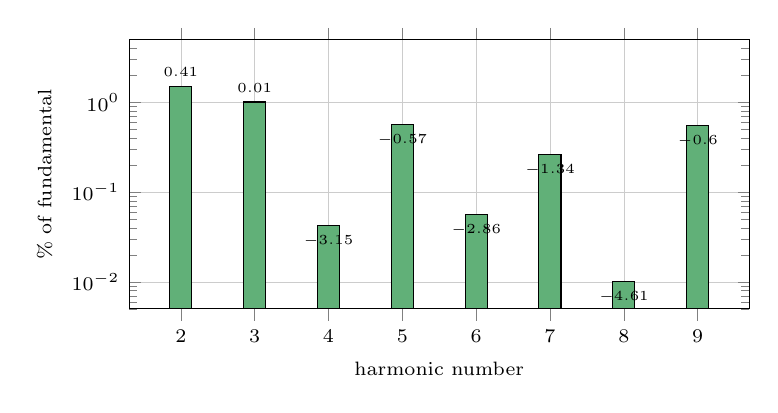
\begin{tikzpicture}
\begin{axis}[width=0.78\textwidth,height=5cm,ybar,bar width=8pt,ymode=log,log origin=infty,ymin=0.005,ymax=5,
  xtick={2,3,4,5,6,7,8,9},xlabel={harmonic number},ylabel={\% of fundamental},grid=major,
  grid style={line width=.2pt,draw=gray!40},tick label style={font=\scriptsize},label style={font=\scriptsize},
  enlarge x limits=0.1,nodes near coords,every node near coord/.append style={font=\tiny,/pgf/number format/.cd,fixed,precision=2}]
\addplot[fill=ctp5!70] coordinates {(2,1.509) (3,1.012) (4,0.043) (5,0.565) (6,0.057) (7,0.261) (8,0.010) (9,0.551)};
\end{axis}
\end{tikzpicture}
\caption{Harmonics of the simulated output. The second harmonic (1.5\,\%) comes mainly from $Q_1$, which swings $\pm$1.5\,mA on a 2\,mA bias; the third (1.0\,\%) is the residual of the piecewise-linear shaping. Total THD = 2.0\,\%.}
\end{figure}

\subsection{Hand calculation versus simulation}
\begin{center}
\small
\begin{tabular}{@{}lcc@{}}
\toprule
Quantity & Hand ($\beta=100$) & Simulation (2N2222) \\
\midrule
Filter capacitor voltage, mean / ripple & 15.9\,V / 0.745\,V$_{pp}$ & 16.13\,V / 0.64\,V$_{pp}$ \\
Regulated rail / ripple & 12\,V / 52\,mV$_{pp}$ & 12.01\,V / 37\,mV$_{pp}$ \\
Supply current of the signal chain & 11.9\,mA & 12.3\,mA \\
Zener current, worst low input (15.81\,V) & 9.4\,mA at 20\,mA load & 19.4\,mA ($>5$\,mA) \\
Zener power, no load, highest input & 427\,mW & 445\,mW ($<1$\,W) \\
$Q_1$: $V_B$, $V_E$, $V_C$, $I_C$ & 1.80, 1.10, 6.92\,V, 1.88\,mA & 1.85, 1.19, 6.49\,V, 2.04\,mA \\
$Q_2$: $V_E$, $I_E$ & 5.97\,V, 2.99\,mA & 6.11\,V, 3.06\,mA \\
$Q_3$: $V_E$, $I_E$ & 4.16\,V, 2.31\,mA & 4.61\,V, 2.56\,mA \\
TP2 triangle & 0.49\,V$_{pp}$ & 0.489\,V$_{pp}$ \\
TP3 amplified triangle & 6.1\,V$_{pp}$ & 6.03\,V$_{pp}$ \\
TP4 shaped & 3.99\,V$_{pp}$ & 3.79\,V$_{pp}$ \\
TP5 output & 3.9\,V$_{pp}$ & 3.76\,V$_{pp}$ \\
THD of TP5 & 1.6\,\% (ideal diodes) & \textbf{2.0\,\%} \\
THD of TP3 (triangle) & 12\,\% (ideal triangle) & 11.6\,\% \\
\bottomrule
\end{tabular}
\end{center}
The 2N2222's higher gain moves the DC levels by up to 0.45\,V ($Q_3$ emitter), but the signal amplitudes agree with the hand design within about 5\,\%. $Q_1$ never clips: its collector swings between 3.4\,V and 9.4\,V.

\subsection{Sensitivity to transistor gain}
\begin{center}
\small
\begin{tabular}{@{}cccccc@{}}
\toprule
$\beta_F$ & $V_{C1}$ & $V_{E2}$ & $V_{E3}$ & TP5 (V$_{pp}$) & THD \\
\midrule
120 & 6.77\,V & 6.00\,V & 4.20\,V & 3.72 & 2.0\,\% \\
256 (2N2222) & 6.49\,V & 6.11\,V & 4.61\,V & 3.76 & 1.9--2.0\,\% \\
350 & 6.42\,V & 6.14\,V & 4.71\,V & 3.77 & 1.8\,\% \\
\bottomrule
\end{tabular}
\end{center}
The output amplitude and distortion barely change over a threefold range of $\beta$, which is what the voltage-divider bias and the AC-coupled shaper are meant to achieve.

\textbf{What I still cannot confirm:} the exact numbers in Multisim (its 2N2222 and 1N4148 models differ slightly from the ones above), resistor and capacitor tolerances, and the transformer's real regulation. Expect a few tenths of a percent of THD difference.

% =====================================================================
\section{Simulation procedure and expected results}
\label{sec:expected}
% =====================================================================
\begin{enumerate}
\item \textbf{Transient analysis:} run 100\,ms or more with a maximum time step of $\le1\,\mu$s. The RC and coupling capacitors need about 30\,ms to settle, so read results from the last few cycles.
\item \textbf{Scope channels:} A = TP1, B = TP3, C = TP4, D = TP5. Use AC coupling on TP3 and TP4 to see the waveform around its 6\,V centre.
\item \textbf{Fourier analysis} on TP5: fundamental 1\,kHz, 9 harmonics; record THD.
\item \textbf{DC operating point:} confirm the Q-points in the table below.
\end{enumerate}

\begin{center}
\small
\begin{tabular}{@{}lll@{}}
\toprule
Item & Hand calculation & Your simulation \\
\midrule
Filter ripple & 0.75\,V$_{pp}$ at 100\,Hz & \rule{2cm}{0.3pt} \\
Regulated rail & 12\,V, ripple $\approx$50\,mV$_{pp}$ & \rule{2cm}{0.3pt} \\
$Q_1$: $V_B$, $V_E$, $V_C$ & 1.8\,V, 1.1\,V, 6.9\,V & \rule{2cm}{0.3pt} \\
$Q_2$: $V_E$ & $\approx$6.0\,V & \rule{2cm}{0.3pt} \\
$Q_3$: $V_E$ & $\approx$4.2\,V & \rule{2cm}{0.3pt} \\
TP2 triangle & $\approx$0.49\,V$_{pp}$ & \rule{2cm}{0.3pt} \\
TP3 triangle & $\approx$6.1\,V$_{pp}$ & \rule{2cm}{0.3pt} \\
TP4 shaped & $\approx$4\,V$_{pp}$ & \rule{2cm}{0.3pt} \\
TP5 sine & 3.8--3.9\,V$_{pp}$, THD 1.6\,\% (model); my 2N2222 simulation: 3.76\,V$_{pp}$, 2.0\,\% & \rule{2cm}{0.3pt} \\
\bottomrule
\end{tabular}
\end{center}

\subsection{Troubleshooting}
\begin{center}
\small
\begin{tabularx}{\textwidth}{@{}>{\raggedright}p{4.1cm}>{\raggedright}p{4.4cm}X@{}}
\toprule
Symptom & Likely cause & Fix \\
\midrule
Triangle looks exponential & $RC$ too small & Increase $R$ or $C$ so $RC\ge5T$ \\
Triangle too small or large & Wrong $RC$ or $Q_1$ gain & Adjust $R_{int}$ (amplitude $\propto1/R$) \\
Flat-topped triangle at TP3 & $Q_1$ clipping & Lower the amplitude or raise $R_{E1}$ \\
Sine still pointy & Taps too far apart or signal too small & Lower tap 1 slightly; check TP3 is $\pm3$\,V \\
Sine too flat & Taps too low & Raise the tap voltages by 0.05--0.1\,V \\
Sine asymmetric, strong 2nd harmonic & Shaper centre differs from the $Q_2$ DC level & Keep $C_{sh}$ and $R_{ref}$; check the 6.00\,V ladder centre \\
$Q_2$ emitter not at 6\,V & $\beta$ differs from 100 & Adjust $R_{B3}$ or $R_{B4}$ slightly \\
Zener output below 12\,V & Zener current too low & Reduce $R_S$ (keep $P_Z<1$\,W) \\
High THD & Too few break points & Add a third diode branch per side \\
\bottomrule
\end{tabularx}
\end{center}
If a stage misbehaves, replace everything after it by a resistor equal to the next stage's input impedance ($Z_{in1}=5.2$\,k$\Omega$, $Z_{in2}=8.7$\,k$\Omega$, $Z_{in3}=37.7$\,k$\Omega$) and debug it alone.

% =====================================================================
\section{Report outline and demonstration plan}
\label{sec:report}
% =====================================================================
\textbf{Report outline}
\begin{enumerate}
\item Title, objective, block diagram (Fig.~\ref{fig:blocks}).
\item Theory: rectification and filtering, Zener regulation, RC integration, clipping shaper, BJT biasing and amplification.
\item Design calculations (Section~3).
\item Complete schematic with test points (Fig.~\ref{fig:full}).
\item Simulation results: rail, every test point, DC operating points, Fourier/THD.
\item Table comparing calculated and simulated values with percentage error.
\item Discussion: error sources, why buffers were added, fixed-frequency limitation.
\item Conclusion and experiment-to-stage mapping.
\end{enumerate}

\textbf{Demonstration (3--5 minutes)}
\begin{enumerate}
\item Show the AC input, the filtered rail and the regulated 12\,V.
\item Run the simulation and walk down the oscilloscope: square, triangle, amplified triangle, shaped wave, sine.
\item Show the Fourier plot and THD; change $R_{int}$ to show the triangle amplitude respond.
\item Optional: show the Exp.\ 07 clamped output.
\end{enumerate}

\subsection*{Assumptions and limitations}
\begin{itemize}
\item Hand design with $\beta=100$, $V_D=0.65$\,V, $V_T=25$\,mV; ideal transformer and function generator.
\item Waveforms in this document are plotted from the hand-calculation model (ideal diodes), not from a circuit simulator. Your simulator will differ slightly.
\item The simulation in Section~\ref{sec:sim} was run with my own Python circuit solver using SPICE-style device parameters, not with Multisim or LTspice. Treat it as an independent check, not as a replacement for your lab simulator.
\item The design is for a fixed 1\,kHz; triangle amplitude falls as frequency rises.
\item The sine is a piecewise-linear approximation (THD of a few percent), not a precision oscillator.
\item The output is inverted relative to the source because $Q_1$ is a common-emitter stage.
\end{itemize}

\end{document}
